\documentclass{beamer}
% \usepackage[retainorgcmds]{IEEEtrantools}
% 
% \setbeamertemplate{enumerate items}[ball]

\usepackage[utf8x]{inputenc}
\usepackage{beamerthemeSzeged}
\usecolortheme{lily}
\usepackage{graphicx}
\usepackage[font={scriptsize,it}]{caption}
\captionsetup[figure]{labelformat=empty}
\usepackage{graphics, setspace}
\usepackage{subfigure}
\usepackage{epsfig}
\usepackage{tikz}
\mode<presentation>{}
\usepackage{bibentry}
\usepackage{multicol}
\usepackage{mathtools}

\usepackage{amsmath,empheq}
\usepackage{xcolor}

\setbeamerfont{title}{family=\rm}
\setbeamercovered{transparent}

\let\oldfootnotesize\footnotesize
\renewcommand*{\footnotesize}{\oldfootnotesize\tiny}
% \usefonttheme{professionalfonts} % using non standard fonts for beamer
% \usefonttheme{structurebold} % default family is serif
%\usepackage{fontspec}
%\setmainfont{Liberation Serif}
%\input{psfig}
\newenvironment{variableblock}[3]{%
  \setbeamercolor{block body}{#2}
  \setbeamercolor{block title}{#3}
  \begin{block}{#1}}{\end{block}}
  
\makeatletter
\setbeamertemplate{footline}
{%
\begin{beamercolorbox}[colsep=1.0pt]{upper separation line foot}
  \end{beamercolorbox}
  \vspace{1pt}
    \hbox{%
    \begin{beamercolorbox}[wd=0.3333\textwidth,  ht=2.5ex, dp=1.125ex]{title in head/foot}%
      \flushleft\usebeamerfont{title in head/foot}\footnotesize \hspace{1pt} Internally Coupled Ears%\insertshorttitle
    \end{beamercolorbox}%
    \begin{beamercolorbox}[wd=0.67\textwidth, ht=2.5ex, dp=1.125ex, center]{title in head/foot}%
      \flushright\usebeamerfont{title in head/foot}\insertframenumber/\inserttotalframenumber\hspace*{2ex}
    \end{beamercolorbox}}
     \begin{beamercolorbox}[colsep=1.0pt]{lower separation line foot}
  \end{beamercolorbox}
}

\setbeamertemplate{headline}
{%
  \begin{beamercolorbox}[ht=3.5ex,dp=1.125ex,%
      leftskip=.3cm,rightskip=.3cm plus1fil]{section in head/foot}
    \usebeamerfont{section in head/foot}\usebeamercolor[fg]{section in head/foot}%
    \flushleft\insertsectionnavigationhorizontal{\textwidth}{}{}
    %\insertsectionhead
  \end{beamercolorbox}%
  \begin{beamercolorbox}[colsep=1.5pt]{middle separation line head}
  \end{beamercolorbox}
  \begin{beamercolorbox}[ht=2.5ex,dp=1.125ex,%
    leftskip=.3cm,rightskip=.3cm plus1fil]{subsection in head/foot}
    \usebeamerfont{subsection in head/foot}\insertsubsectionhead %\ - \insertsubsubsectionhead
  \end{beamercolorbox}%
  \begin{beamercolorbox}[colsep=1.5pt]{lower separation line head}
  \end{beamercolorbox}
}

\setbeamertemplate{blocks}[rounded][shadow=false]
\addtobeamertemplate{block begin}{\pgfsetfillopacity{0.8}}{\pgfsetfillopacity{1}}
\setbeamercolor*{block title example}{fg=blue!75,bg= blue!10}
\setbeamercolor*{block body example}{fg= black,bg= blue!5}
\setbeamercolor{frametitle}{fg=blue}
\beamertemplatenavigationsymbolsempty
\makeatother

\title{\Large Mechanical Processing in Internally Coupled Ears}
\author{Anupam Prasad Vedurmudi}
\date{TMP Thesis Defence\\ \today}

\titlegraphic{\vspace{.1cm}\flushleft 
\includegraphics[width=.85cm]{Diagrams/T35logo2.png}\hspace*{8.3cm}~%
   
\includegraphics[width=2cm]{Diagrams/tmplogo.jpg}
}

\AtBeginSection[]
{
  \begin{frame}<beamer>
    \frametitle{Outline for Section \thesection}
    \begin{multicols}{2}
    \tableofcontents[currentsection,subsubsectionstyle=show/shaded]
    \end{multicols}
  \end{frame}
}

% \titlegraphic{\vspace{8cm}}
\begin{document}

\begin{frame}[t]
%    \tikz [remember picture,overlay]
%     \node at
%         ([yshift=3cm]current page.south) 
%         %or: (current page.center)
%         {\includegraphics[width=\textwidth,height=.5\textheight]{someimage}};
   %\titlepage
 \titlepage
 \bibliographystyle{ieeetr}
\nobibliography{literatur}

\end{frame}

%\logo{
\includegraphics[height=0.8cm]{Diagrams/T35logo2.png}\vspace{220pt}}

\section{Introduction}
\subsection{Auditory Systems}
\begin{frame}[t]
\frametitle{Auditory Systems}

 \begin{columns}
 
     \begin{column}{0.5\textwidth}
    \centering
    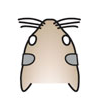
\includegraphics[width = 1.5 cm]{Diagrams/Presentation/indepears.png}\\
    \end{column}
     
    \begin{column}{0.5\textwidth}
    \centering
    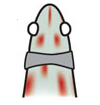
\includegraphics[width = 1.5 cm]{Diagrams/Presentation/coupledears.png}\\
    \end{column}
    
  \end{columns}
  
 \begin{columns}
     \begin{column}{0.5\textwidth}
    \centering
    \underline{\textbf{Independent Ears}}
    \end{column}
     
    \begin{column}{0.5\textwidth}
    \centering
    \underline{\textbf{Coupled Ears}}
    \end{column}
  \end{columns}

  \begin{columns}
    \begin{column}{0.5\textwidth}
    \centering
%     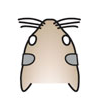
\includegraphics[width = 1.5 cm]{Diagrams/Presentation/indepears.png}\\
%     \underline{\textbf{Independent Ears}}
    \small
     \begin{itemize}
     \item[]
    \item[] Eustachian tubes generally very narrow.
     \item[] Effectively independent eardrum vibrations.
     \end{itemize}
    \end{column}
     
    \begin{column}{0.5\textwidth}
    \centering
%     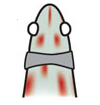
\includegraphics[width = 1.5 cm]{Diagrams/Presentation/coupledears.png}\\
%     \underline{\textbf{Coupled Ears}}
    \small
     \begin{itemize}
         \item[] Wide eustachian tubes open into the mouth cavity.
     \item[] Eardrums vibrations influence eachother.
     \end{itemize}
    \end{column}
    
  \end{columns}
\end{frame}

\subsection{Hearing Cues}
\begin{frame}[t]
 \frametitle{Binaural Hearing Cues}
 %Localization using frequency dependent phase and amplitude differences between the ears.
 %\vspace{\baselineskip}
 \begin{exampleblock}
  \onslide<1->{\begin{columns}
 
    \begin{column}{0.5\textwidth}
    \centering
    \underline{\textbf{Interaural Time Difference}}

    \end{column}
     
    \begin{column}{0.5\textwidth}
    \centering
    \underline{\textbf{Interaural Level Difference}}
    \end{column}
    
  \end{columns}
  
    \begin{columns}
 
    \begin{column}{0.5\textwidth}
    %\centering
    \small
     \begin{itemize}
%      \item[]
    \item[] Phase difference between the (pressure) inputs to the ears.
    \item ITD
     %\item[] Effectively independent eardrum vibrations.
     \end{itemize}
    \end{column}
     
    \begin{column}{0.5\textwidth}
    %\centering
    \small
     \begin{itemize}
          \item[] Amplitude difference between the inputs.
          \item ILD
     %\item[] Eardrums vibrations influence eachother.
     \end{itemize}
    \end{column}
    
  \end{columns}}
  \end{exampleblock}  
  \vfill
  \begin{exampleblock}{}
  \onslide<2->{\begin{columns}
 
    \begin{column}{0.5\textwidth}
    \centering
    \underline{\textbf{Internal Time Difference}}

    \end{column}
     
    \begin{column}{0.5\textwidth}
    \centering
    \underline{\textbf{Internal Level Difference}}
    \end{column}
    
  \end{columns}
  
    \begin{columns}
 
    \begin{column}{0.5\textwidth}
    %\centering
    \small
     \begin{itemize}
%      \item[]
    \item[] Phase difference between the eardrum vibrations.
    \item iTD
     %\item[] Effectively independent eardrum vibrations.
     \end{itemize}
    \end{column}
     
    \begin{column}{0.5\textwidth}
    %\centering
    \small
     \begin{itemize}
          \item[] Amplitude difference between the vibrations.
          \item iLD
     %\item[] Eardrums vibrations influence eachother.
     \end{itemize}
    \end{column}
    
  \end{columns}}
  \end{exampleblock}
\end{frame}


\begin{frame}[t]
 \begin{exampleblock}{Advantages of Coupled Ears}
 \begin{itemize}
  \item Low frequencies result in reduced degradation of hearing cues in dense enviroments.
 \end{itemize}

  
 \end{exampleblock}

\end{frame}

\begin{frame}[t]
 \frametitle{ICE Model}
\begin{exampleblock}{}
 \begin{itemize}
  \item[] Based on the model first presented by Vossen\footnote{\bibentry{vossenjasa}}.
 \end{itemize}

\end{exampleblock}

\end{frame}

\section{The Model}

\subsection{Mouth Cavity}
\begin{frame}[t]
\frametitle{Mouth Cavity}
% \begin{figure}[htl]
% \flushleft
% 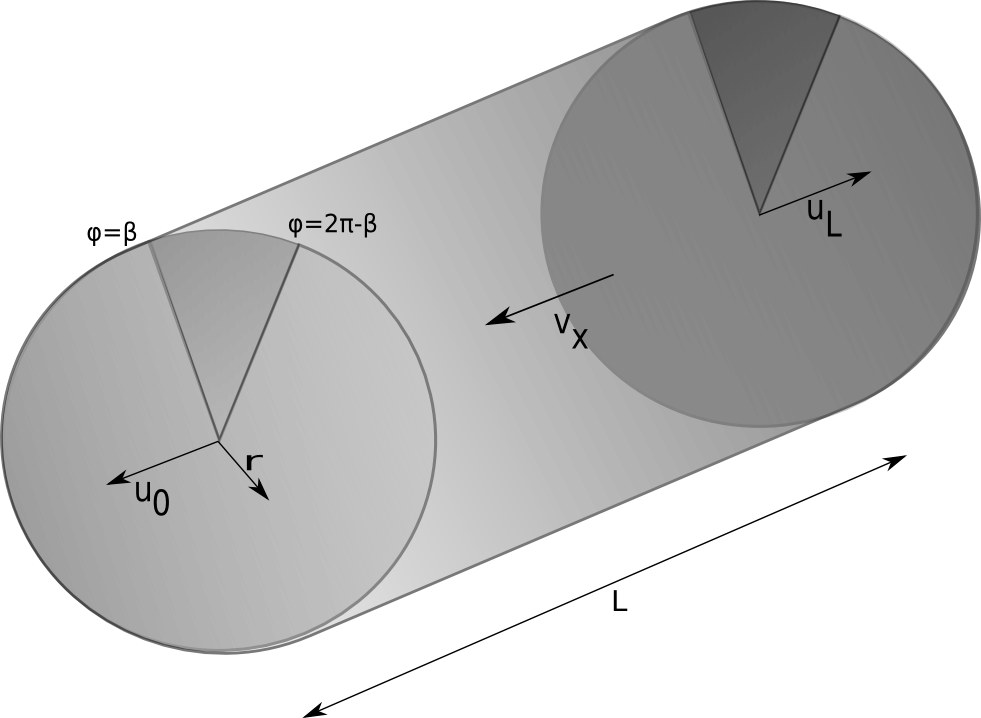
\includegraphics[width=.36\textwidth]{Diagrams/oldCylinder.png}
% %\caption{Previous Cylindrical Cavity}
% \end{figure}
% \begin{figure}[htr]
% 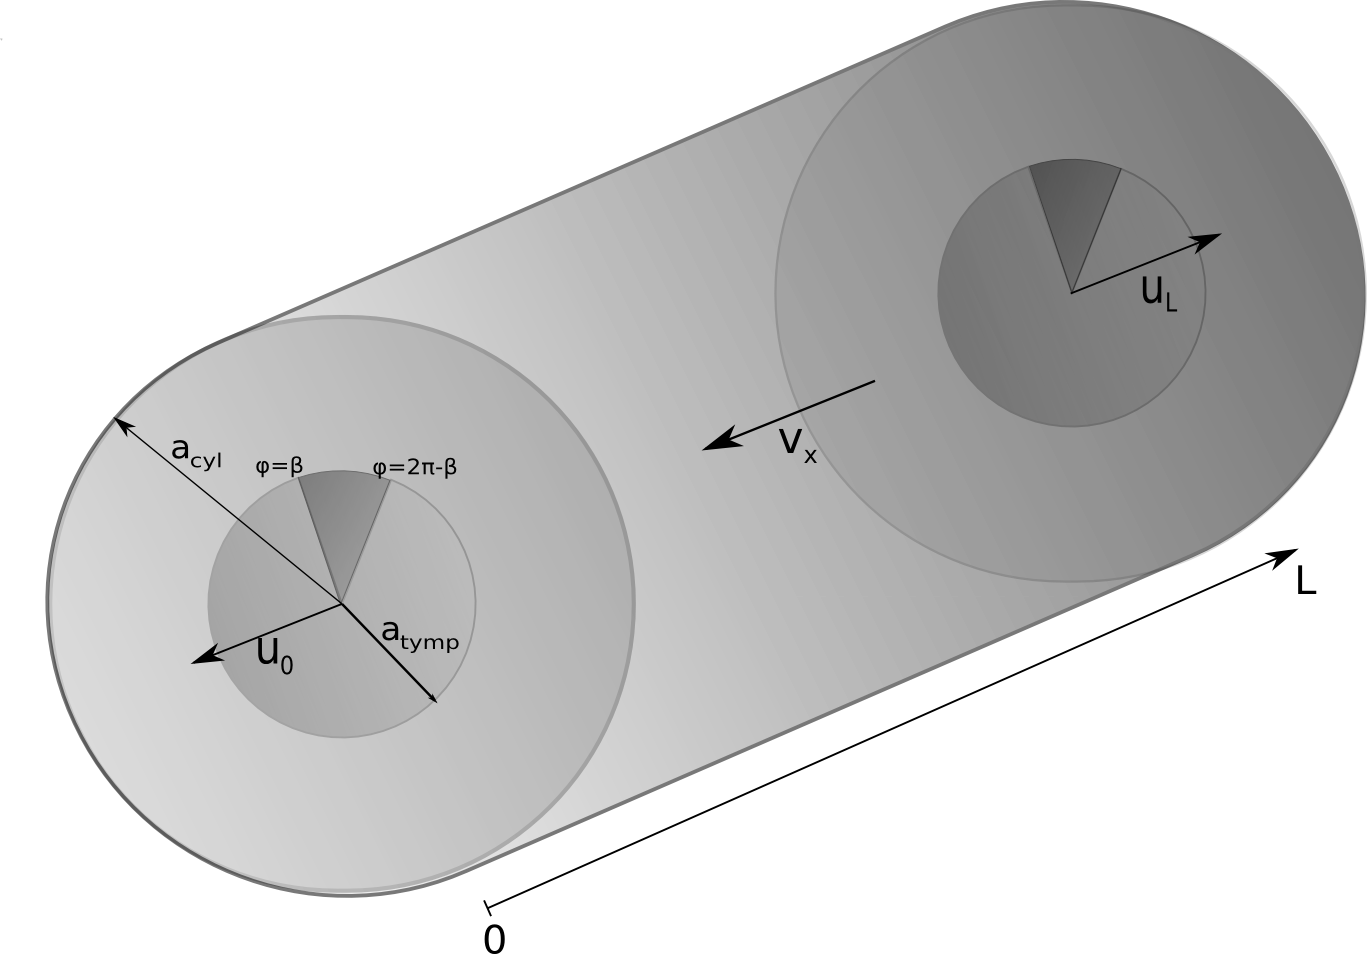
\includegraphics[width=.38\textwidth]{Diagrams/newCylinder.png}
% \caption{Mouth Cavity Model}
% \end{figure}
\begin{columns}

 \begin{column}{0.5\textwidth}
   \onslide<1->{
   \footnotesize
    \underline{\textbf{Previous Model}}\\
    \centering
    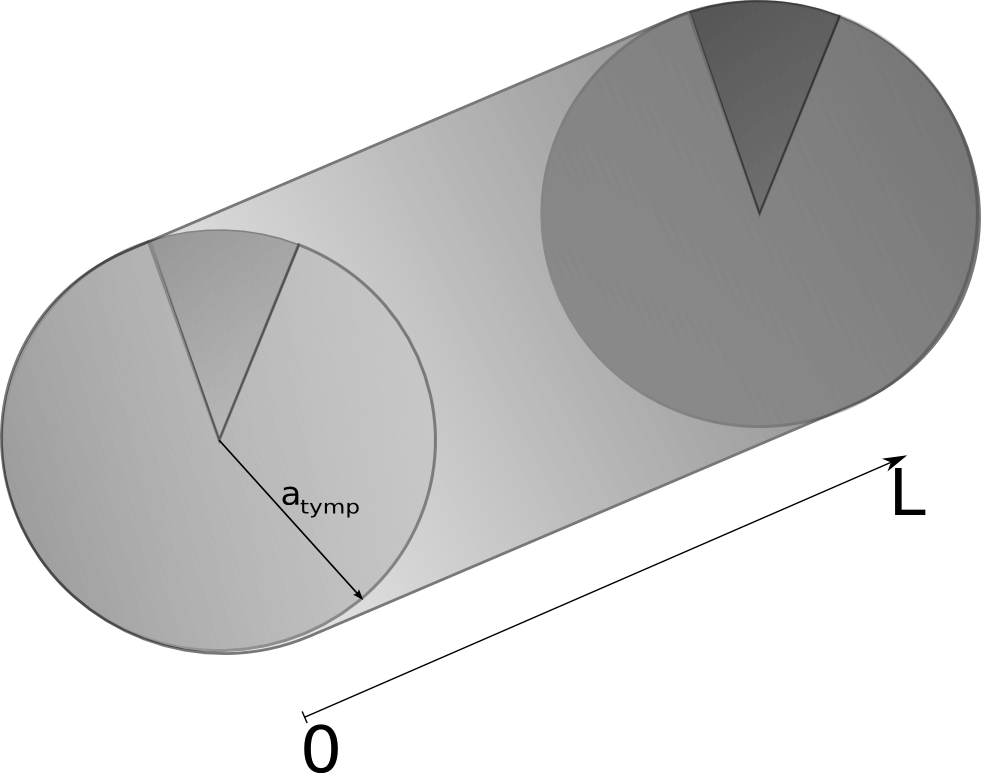
\includegraphics[width = 4 cm]{Diagrams/Presentation/oldCylinder.png}\\
    \small
    \begin{exampleblock}{ }
    \begin{itemize}
     \item[] $a_{\mathrm{tymp}}$ fixed.
     \item[] $V_{\mathrm{cyl}}=\pi a^2_{\mathrm{tymp}}L$
    \end{itemize}
    \end{exampleblock}}

    \end{column}
    
 \begin{column}{0.5\textwidth}
    \onslide<2->{
        \footnotesize
    \underline{\textbf{Our Model}}\\
    \centering
    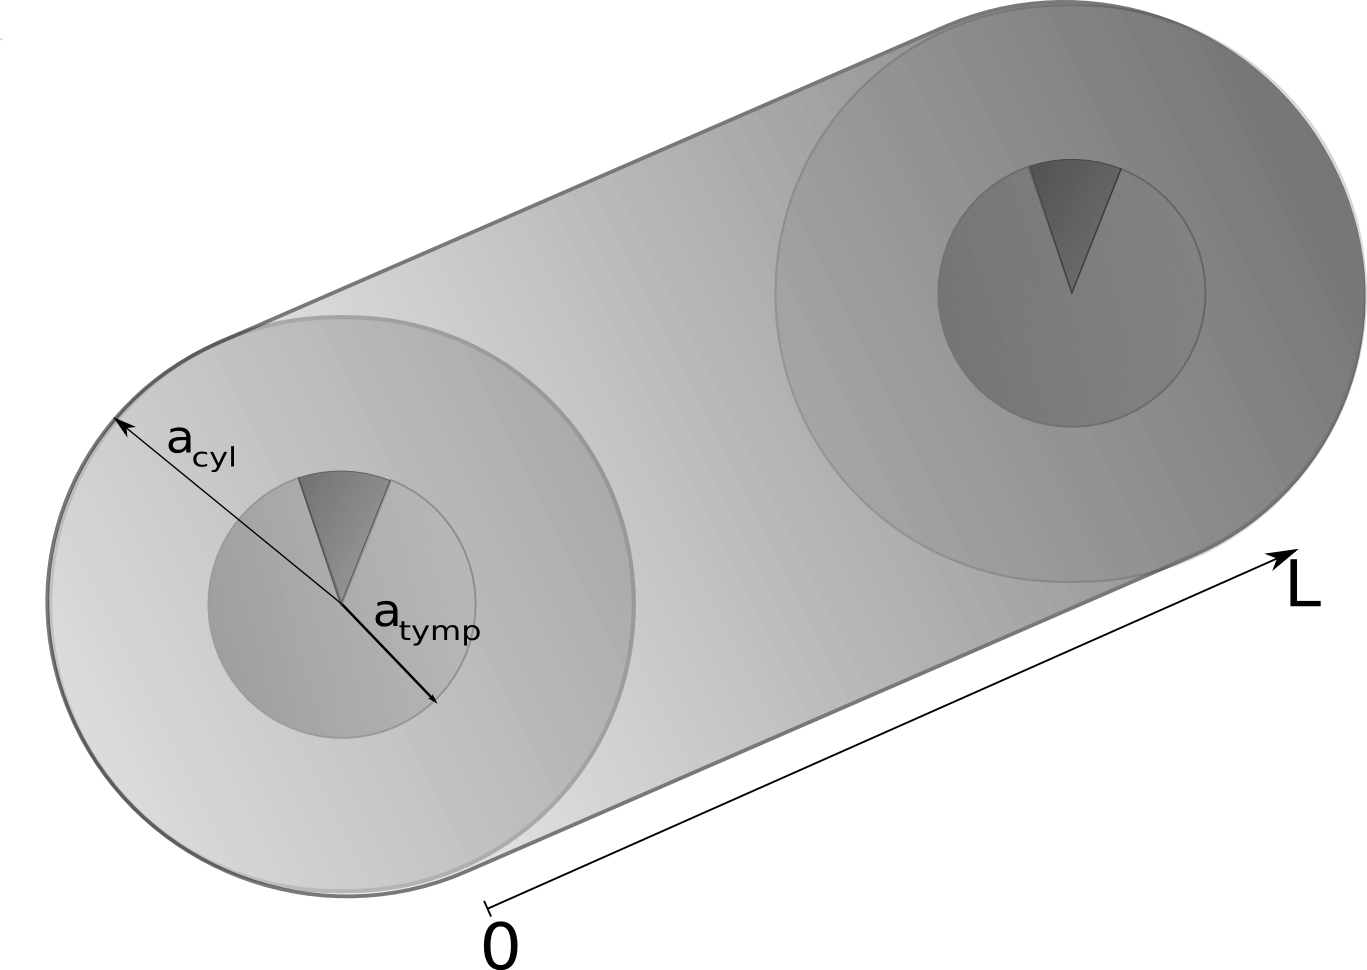
\includegraphics[width = 4 cm]{Diagrams/Presentation/newCylinder.png}\\
    \small
    \begin{exampleblock}{ }
    \begin{itemize}
     \item[] $a_{\mathrm{tymp}},\ V_{\mathrm{cyl}}$ fixed. 
     \item[] $a_{\mathrm{cyl}}=\sqrt{V_{\mathrm{cyl}}/\pi L}$
    \end{itemize}
    \end{exampleblock}}
    \end{column}
    
    \end{columns}
\end{frame}

\subsubsection{Acoustic Head Model}
\begin{frame}[t]
 \frametitle{Acoustic Head Model}
 \begin{columns}
     \begin{column}{.5\textwidth}
    \small
    \flushleft
     \begin{itemize}
      \item<1> \textbf{I} - Ipsilateral ear, \textbf{C} - Contralateral ear.
      \item<1>  $p_0,\ p_L$ - sound pressure on eardrums,
      $\theta$ - sound source direction.
     \end{itemize}
     
     \begin{itemize}
      \item<2> Sound source ``far away''.
      \item<2> No appreciable amplitude difference, $|p_0|=|p_L|$.
      \item<2> Phase difference between sound at both ears - $\Delta=kL\sin\theta$.
      \item<3> $p_0=pe^{j\omega t -.5kL\sin\theta}$\\ $p_L=pe^{j\omega t +.5kL\sin\theta}$
      \end{itemize}

    \end{column}
    
 \begin{column}{0.5\textwidth}
%     \centering
%     \small
%     \underline{\textbf{Head Model}}\\
%     \flushleft
    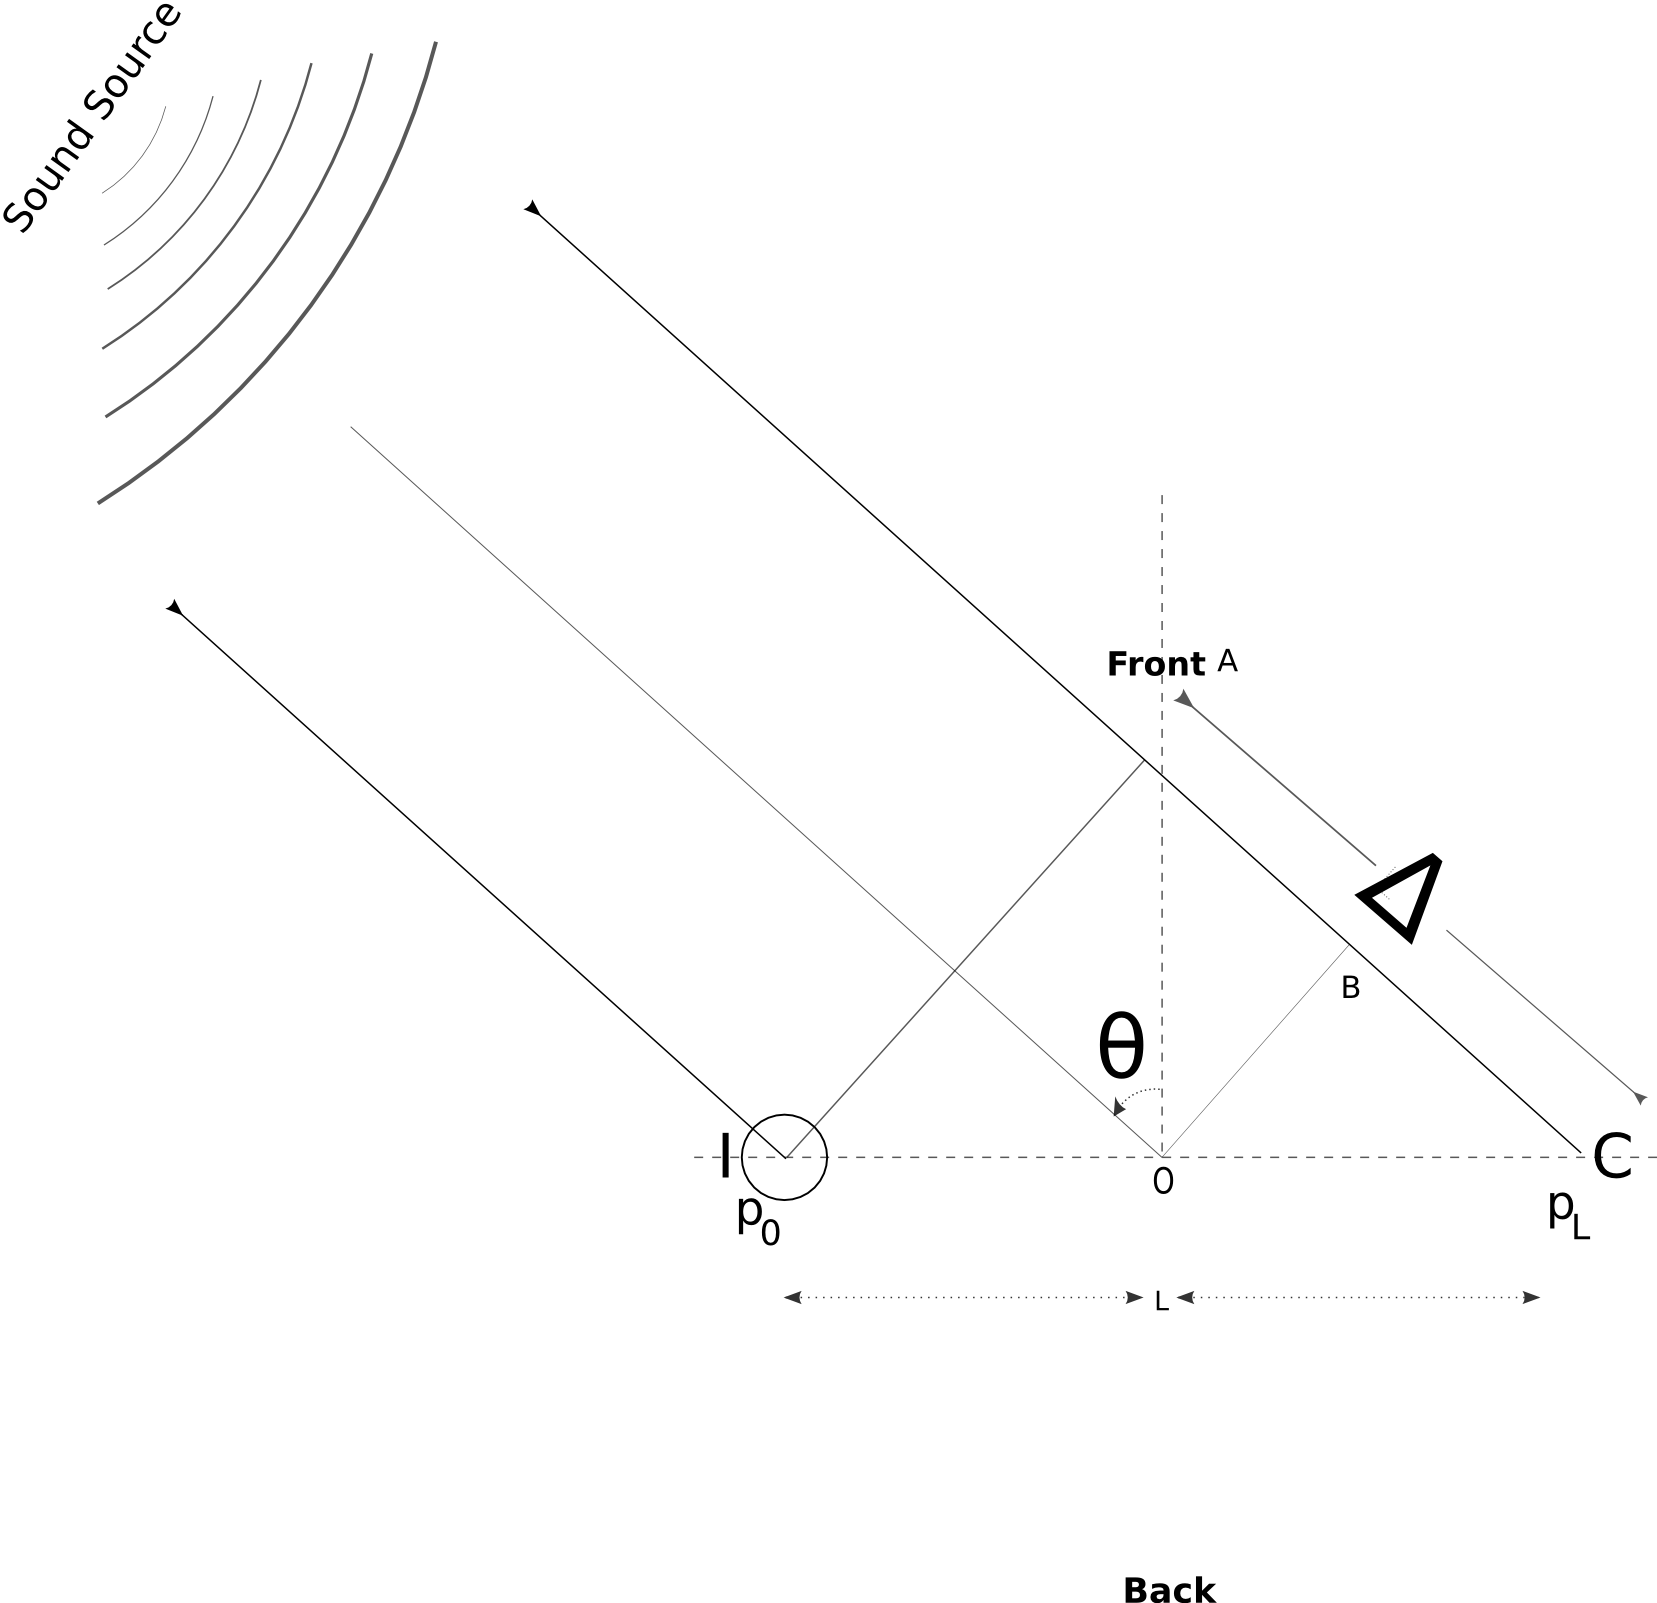
\includegraphics[width = 6 cm]{Diagrams/Presentation/acousticheadmodelold.png}\\
    \end{column}

    \end{columns}
\end{frame}

\begin{frame}[t]
 \frametitle{Acoustic Head Model contd.}
 \begin{columns}
     \begin{column}{.5\textwidth}
    \small
    \flushleft
%      \begin{itemize}
%       \item<1> \textbf{I} - Ipsilateral ear, \textbf{C} - Contralateral ear.
%       \item<1>  $p_0,\ p_L$ - sound pressure on eardrums,
%       $\theta$ - sound source direction.
%      \end{itemize}
     \begin{itemize}
      \item $|p_0|=|p_L|$.
      \item Increased  phase difference due to diffraction - $\Delta=1.5kL\sin\theta$.
      \item $p_0=pe^{j\omega t -.75kL\sin\theta}$\\ $p_L=pe^{j\omega t +.75kL\sin\theta}$
      \end{itemize}

    \end{column}
    
 \begin{column}{0.5\textwidth}
%     \centering
%     \small
%     \underline{\textbf{Head Model}}\\
%     \flushleft
    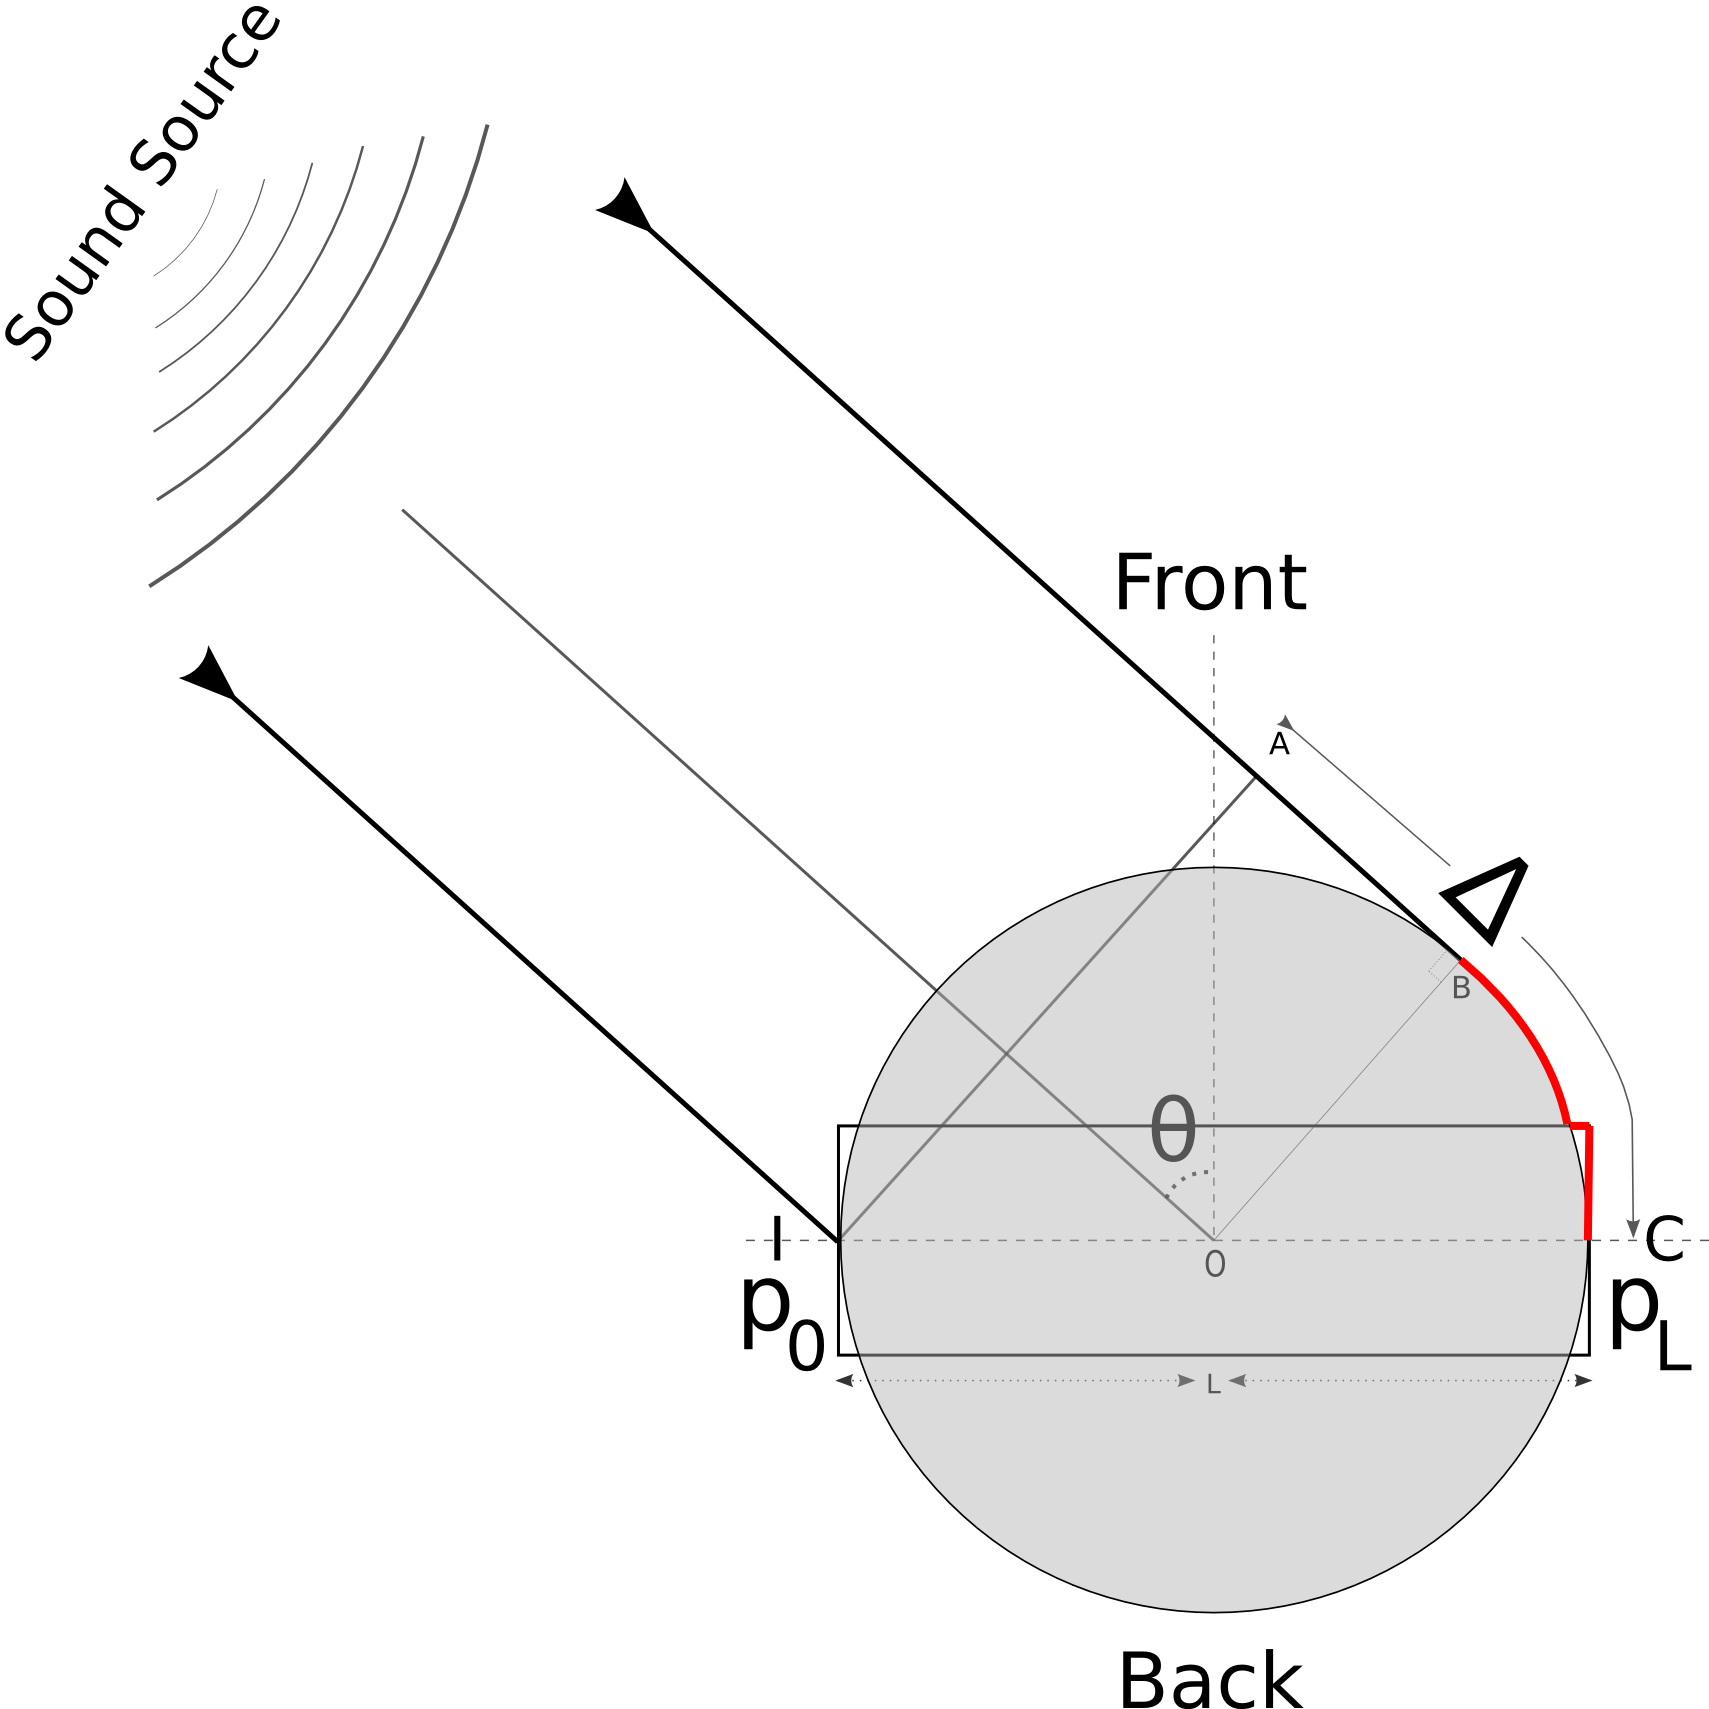
\includegraphics[width = 6 cm]{Diagrams/Presentation/acousticheadmodel2.png}\\
    \end{column}

    \end{columns}
\end{frame}

\subsubsection{Pressure Derivation}
\begin{frame}[t]
\frametitle{Cavity Pressure}
\begin{exampleblock}{3D Wave Equation}
\begin{equation}\label{pressurewaveeqn}
\begin{split}
 \frac{1}{c^2}\partial^2_t p(x,r,\phi,t)=\frac{1}{r}\frac{\partial}{\partial r}&\left(r\frac{\partial p(x,r,\phi,t)}{\partial r}\right)
 \\&+\frac{1}{r^2}\frac{\partial^2 p(x,r,\phi,t)}{\partial \phi^2}
 +\frac{\partial p(x,r,\phi,t)}{\partial x^2}
 \end{split}
\end{equation}
\end{exampleblock}
\begin{variableblock}{}{bg= blue!5,fg=black}{bg= blue!5,fg=blue!75}
 To be solved using the separation ansatz \[p(x,r,\phi,t)=f(x)g(r)h(\phi)e^{j\omega t}.\]
\end{variableblock}

% Subject to the no-penetration boundary condition at all solid boundaries.

\end{frame}

% \begin{frame}[t]
% \frametitle{Eardrum}
% %  \begin{figure}[ht!]
% %   \centering
% %   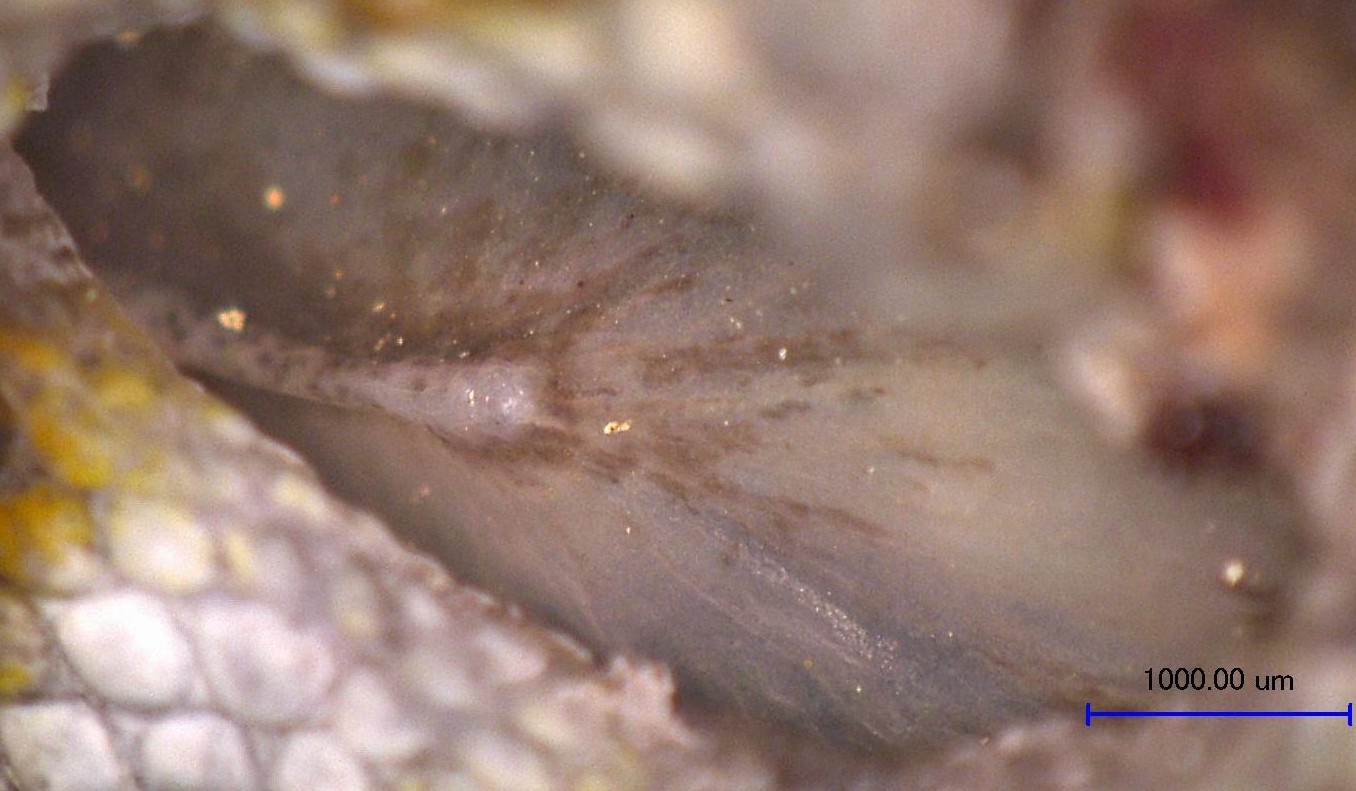
\includegraphics[width=.34\textwidth]{Diagrams/geckoextracolumella2.jpg}
% % \end{figure}
% \begin{figure}[htb!]
% \makebox[\linewidth]{
% 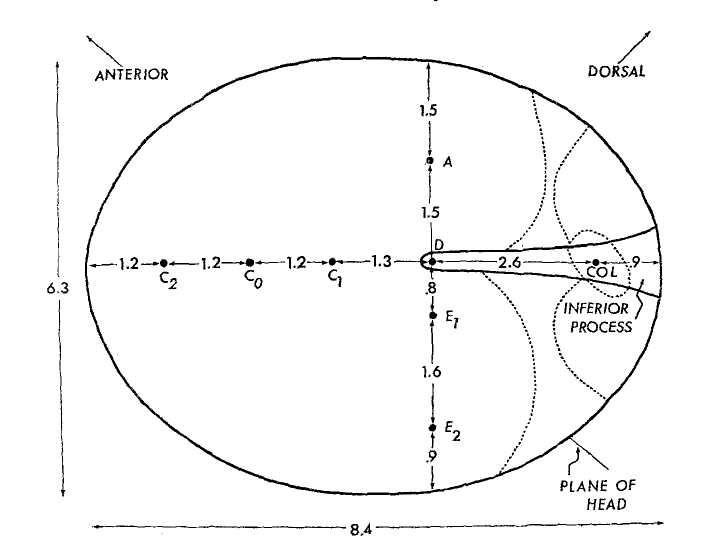
\includegraphics[width=.37\textwidth]{Diagrams/geckoear.png}
% \hfill
% 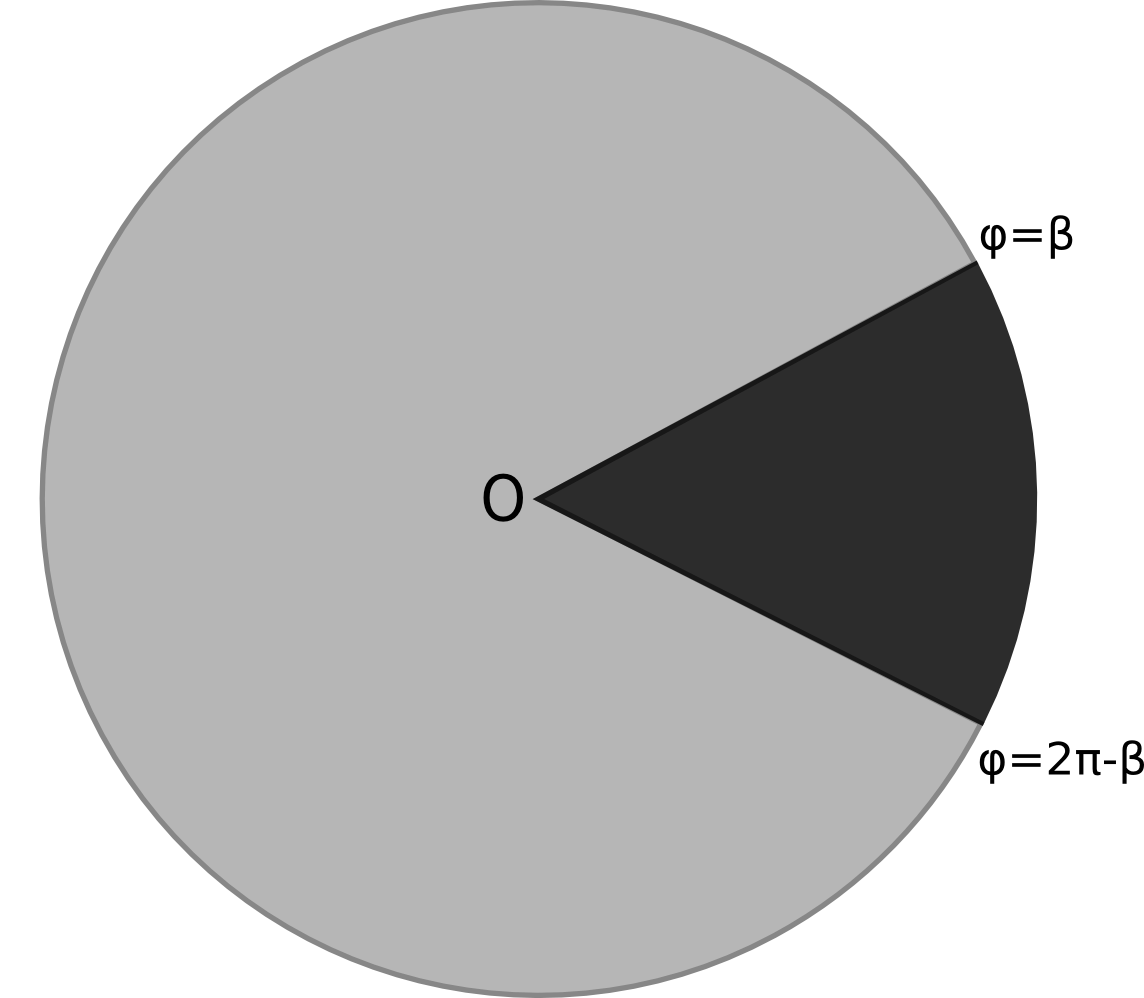
\includegraphics[width=.3\textwidth]{Diagrams/tympanummodel.png}}
% 
% \end{figure}
% 
% \end{frame}

\begin{frame}[t]
\frametitle{Separated Equations}
\onslide<1->{\begin{exampleblock}{$x$- and $\phi$- directions}
 \begin{align}
 \frac{d^2 f(x)}{dx^2}+\zeta^2f(x)=0\longrightarrow f(x)=e^{\pm j\zeta x}\\
 \frac{d^2 h(\phi)}{d\phi^2}+q^2h(\phi	)=0\longrightarrow h(\phi)=e^{\pm jq\phi}
 \end{align}
\end{exampleblock}}

\onslide<2->{\begin{exampleblock}{$r$-direction, Bessel functions}
 \begin{equation}
 \begin{split}
  \frac{1}{r}\frac{\partial}{\partial r}\left(r\frac{\partial g(r)}{\partial r}\right)+\left[\nu^2-\frac{q^2}{r^2}\right]g(r)=0
  &\longrightarrow g(r) = J_q(\nu r)\\
  &\mbox{where, } \nu^2=k^2-\zeta^2
  \end{split}
 \end{equation}
\end{exampleblock}}

\end{frame}

\begin{frame}[t]
 \frametitle{Boundary Conditions - $\phi$}
 \begin{exampleblock}{Smoothness and Continuity in $\phi$.}
  \begin{align}
   \phi&\rightarrow h(0)=h(2\pi)\quad\mbox{and}\quad h^\prime(0)=h^\prime(2\pi)\nonumber\\
   \mbox{}\nonumber\\
   &\Rightarrow h(\phi)=\cos q\phi,\ q=0,1,2,\ldots
  \end{align}
 \end{exampleblock}
\end{frame}

\begin{frame}[t]
 \frametitle{Boundary Conditions - $r$}
 \begin{exampleblock}{Impenetrable boundary at $r=a_{\mathrm{cyl}}$, i.e. normal derivative vanishes}
\begin{equation}
 -j\rho\omega\mathbf{v}=\mathbf{n}.\left.\nabla p(x,r,\phi;t)\right|_{r=a_{\mathrm{cyl}}}\equiv\left.\frac{\partial g}{\partial r}\right|_{r=a_{\mathrm{cyl}}}=0
\end{equation}
\begin{align}
 \Rightarrow g(r)=J_q(\nu_{\mathrm{qs}}r/a_{\mathrm{cyl}})
\end{align}
\end{exampleblock}

\begin{variableblock}{Bessel Prime Zeros}{bg= blue!5,fg=black}{bg= blue!5,fg=blue!75}
\begin{itemize}
 \item $\nu_{\mathrm{qs}}$ - zeros of $J^\prime_q$, $s=0,1,2,\ldots$
 \item $\nu_{\mathrm{00}}$=0
 \end{itemize}
\end{variableblock}


\end{frame}

% \left.\frac{\partial J_q(\nu_{\mathrm{qs}}r)}{\partial r}\right|_{r=a_{\mathrm{cyl}}}=0

\begin{frame}[t]
\frametitle{General Solution}
 \onslide<1>{\begin{exampleblock}{Pressure Modes}
  \begin{align}
   &p(x,r,\phi,t)=\displaystyle\sum^{\infty}_{q=0,s=0}\left[A_{\mathrm{qs}}e^{j\zeta_{\mathrm{qs}}x}+B_{\mathrm{qs}}e^{-j\zeta_{\mathrm{qs}}x}\right]p_{\mathrm{qs}}(r,\phi)e^{j\omega t}\\
   &p_{\mathrm{qs}}(r,\phi)=\cos q\phi J_q(\nu_{\mathrm{qs}}r/a_{\mathrm{cyl}})\\
   &\mbox{where, }  \zeta_{\mathrm{qs}}=\sqrt{k^2-\nu^2_{\mathrm{qs}}/a^2_{\mathrm{cyl}}}\nonumber
  \end{align}
 \end{exampleblock}}
\onslide<2>{\begin{variableblock}{Plane Wave Mode}{bg= blue!5,fg=black}{bg= blue!5,fg=blue!75}
 \begin{equation}
  p_{\mathrm{pw}}(x,r,\phi;t)=\left[A_{00}e^{jkx}+B_{00}e^{-jkx}\right]e^{j\omega t}
 \end{equation}
\end{variableblock}
}
\end{frame}

\subsection{Eardrum}
\subsubsection{Model}
\begin{frame}[t]
\frametitle{Eardrum}
\begin{columns}
    \begin{column}{0.5\textwidth}
      \centering
      \small
      Sketch of a Tokay eardrum as seen from the outside\footnote{\bibentry{manleygecko1}}.\\
      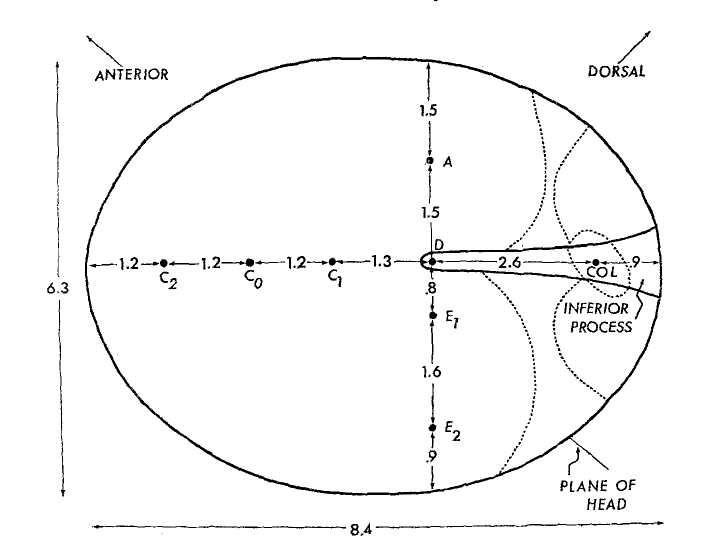
\includegraphics[width = 3.7 cm]{Diagrams/geckoear.png}\\
      \footnotesize
     COL - approximate position opposite the extracolumella insertion.
    \end{column}

    \begin{column}{0.5\textwidth}
      \centering
      \small
      The ICE eardrum.\\
      \textbf{}\\
      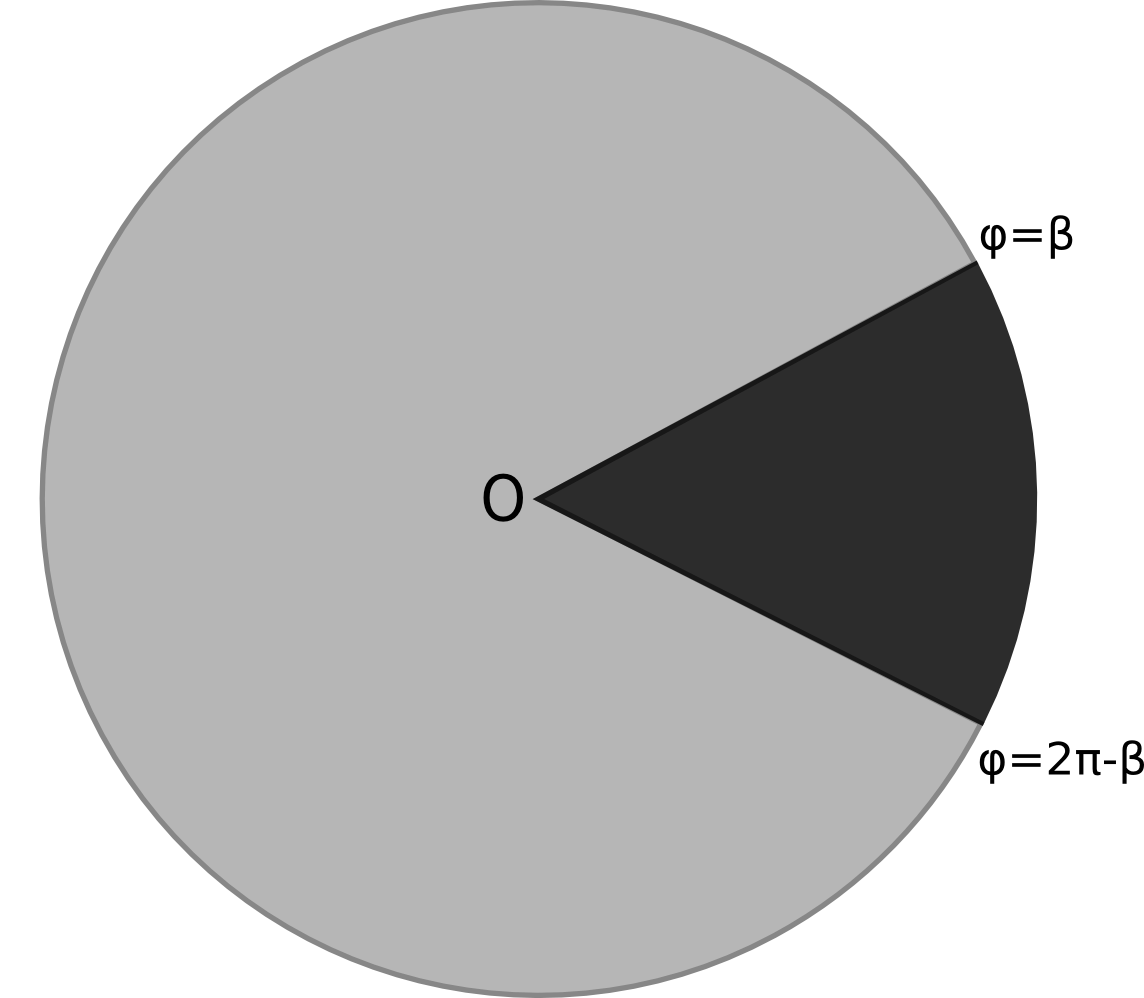
\includegraphics[width = 3.2 cm]{Diagrams/tympanummodel.png}\\
%       \textbf{}\\
%       Extracolumella (dark region) is rigid and stationary.\\
%       \textbf{}\\
%       The membrane material is assumed to be linear elastic.
\footnotesize
\begin{itemize}
      \item[] Extracolumella (dark) - rigid, stationary.
      \item[] Tympanum - assumed linear elastic.
      \item[] Rigidly clamped at the boundaries ($r=a_{\mathrm{tymp}}$ and $\phi=\beta,\ 2\pi-\beta$)
\end{itemize}

    \end{column}
  \end{columns}
  
\end{frame}

\subsubsection{Membrane Vibrations}

\begin{frame}[t]
 \frametitle{Membrane Vibrations}
\begin{exampleblock}{Membrane EOM}

\begin{equation}\label{membraneequation1}
\begin{split}
 -\partial^2_tu(r,\phi;t)-2\alpha\partial_t u(r,\phi;t)+c^2_M\Delta_{(2)}&u(r,\phi;t)=\\ 
 & \frac{1}{\rho_m d}\Psi(r,\phi;t)
 \end{split}
\end{equation}
 \end{exampleblock}

\begin{variableblock}{Membrane parameters}{bg= blue!5,fg=black}{bg= blue!5,fg=blue!75}
  \begin{tabular}{l l}
    $\alpha$ - damping coefficient, & $c^2_M$ - propagation velocity\\
    \hspace{1pt}\\
    $\rho_m$ - density, & $d$ - thickness.
  \end{tabular}
 \end{variableblock}

\end{frame}

\begin{frame}[t]
 \frametitle{Free-Undamped Membrane, $\alpha\rightarrow 0$, $\Psi\rightarrow 0$}
% \onslide<1->{\begin{exampleblock}{Membrane EOM}
% 
% \begin{equation}\label{membraneequation1}
% \begin{split}
%  -\partial^2_tu(r,\phi;t)-2\alpha\partial_t u(r,\phi;t)+c^2_M\Delta_{(2)}&u(r,\phi;t)=\\ 
%  & \frac{1}{\rho_m d}\Psi(r,\phi;t)
%  \end{split}
% \end{equation}
%  \end{exampleblock}}
% 
\begin{variableblock}{Separation Ansatz}{bg= blue!5,fg=black}{bg= blue!5,fg=blue!75}
\begin{equation}\label{mseparationansatz}
 u(r,\phi;t)=f(r)g(\phi)h(t)
\end{equation}
% Same set of equations as in the pressure case.
\end{variableblock}
\begin{exampleblock}{Separated Equations}
 \begin{align}
   \frac{d^2 g(\phi)}{d\phi^2}+\kappa^2g(\phi)&=0\\
   \frac{1}{r}\frac{\partial}{\partial r}\left(r\frac{\partial f(r)}{\partial r}\right)+\left[\mu^2-\frac{\kappa^2}{r^2}\right]f(r)&=0\\
 \frac{d^2 h(t)}{dt^2}+c^2_M\mu^2h(t)&=0
\end{align}
\end{exampleblock}


\end{frame}

\begin{frame}[t]
 \frametitle{Boundary Conditions}
 \onslide<1->{\begin{exampleblock}{$\phi$-direction: $u(r,\beta;t)=u(r,2\pi-\beta,t)=0$}
  \begin{align}
  \Rightarrow &g(\phi)=\sin\kappa(\phi-\beta)\\
  \mbox{where, }&\kappa=\frac{m\pi}{2(\pi-\beta)},\quad m=1,2,3,\ldots\nonumber
  \end{align}
 \end{exampleblock}}
 \onslide<2->{\begin{exampleblock}{$r$-direction: $u(a_{\mathrm{tymp}},\phi;t)=0$}
  \begin{align}
  \Rightarrow &f(r)=J_\kappa(\mu_{\mathrm{mn}}r/a_{\mathrm{tymp}})\\
  \mbox{where, }&\mu_{\mathrm{mn}} \mbox{ is the } n^{\mathrm{th}} \mbox{ zero of } J_\kappa\nonumber
  \end{align}
 \end{exampleblock}}

\end{frame}

\begin{frame}[t]
 \frametitle{}
 \onslide<1->{\begin{exampleblock}{Free eigenmodes}
  \begin{align}
  &u_{\mathrm{mn}}(r,\phi)=\sin \kappa(\phi-\beta) J_\kappa(\mu_{\mathrm{mn}} r)\\
  &u_{\mathrm{free}}(r,\phi;t)=\displaystyle\sum^\infty_{m=0,n=1}C_\mathrm{mn}u_{\mathrm{mn}}(r,\phi)e^{j\omega_{\mathrm{mn}} t}\\
  &\mbox{where, }\omega_{\mathrm{mn}}=c_M\mu_{\mathrm{mn}}\nonumber
  \end{align}
 \end{exampleblock}}
\onslide<2->{\begin{exampleblock}{Damped membrane}
              \begin{equation}
               \widetilde{u}_{\mathrm{free}}(r,\phi;t)=\displaystyle\sum^\infty_{m=0,n=1}\widetilde{C}_{\mathrm{mn}}u_{\mathrm{mn}}(r,\phi)e^{j\omega_{\mathrm{mn}} t-\alpha t}
              \end{equation}
             \end{exampleblock}}
\end{frame}

\begin{frame}[t]
 \frametitle{Forced Vibrations: $\Psi=pe^{j\omega t}$ }
 \onslide<1->{\begin{exampleblock}{Steady State Solution}
  \begin{equation}
  u_{\mathrm{ss}}(r,\phi;t)=:\displaystyle\sum^\infty_{m=0,n=1}C_{\mathrm{mn}}u_{\mathrm{mn}}(r,\phi)e^{j\omega t}
  \end{equation}
  Substitute $u_{\mathrm{ss}}$ in Membrane EOM.
 \end{exampleblock}}
 \onslide<2->{\begin{variableblock}{}{bg= blue!5,fg=black}{bg= blue!5,fg=blue!75}
               \begin{align}
               &C_{\mathrm{mn}}=\frac{p\int dS u_{\mathrm{mn}}}{\Omega_{\mathrm{mn}}\int dS u^2_{\mathrm{mn}}}\\
                &\Omega_{\mathrm{mn}}=\rho_M d \left[(\omega^2-\omega^2_{\mathrm{mn}})-2j\alpha\omega\right]\nonumber
               \end{align}

              \end{variableblock}}

\end{frame}
\begin{frame}[t]
\frametitle{Forced Vibrations contd.}
 \begin{exampleblock}{Transient Solution}
Same as the solution for a free damped membrane
              \begin{equation}
               u_{\mathrm{t}}(r,\phi;t)=\displaystyle\sum^\infty_{m=0,n=1}\widetilde{C}_{\mathrm{mn}}u_{\mathrm{mn}}(r,\phi)e^{j\omega_{\mathrm{mn}} t-\alpha t}
               \end{equation}
$\widetilde{C}_{\mathrm{mn}}$ determined from the membrane displacement at $t=0$.

\noindent $u_{\mathrm{t}}\rightarrow 0$ exponentially as $t\rightarrow\infty$.
\end{exampleblock}
\onslide<2->{\begin{variableblock}{Steady State Approximation}{bg= blue!5,fg=black}{bg= blue!5,fg=blue!75}
\centering $u\approx u_{\mathrm{ss}}\mbox{ if } \alpha \mbox{ is ``large'' }$.
\end{variableblock}}

\end{frame}

\subsection{Coupled Membranes}
\subsubsection{Ansatz}
\begin{frame}
 \frametitle{Coupled Membranes}
 \onslide<1->{\begin{variableblock}{}{bg= blue!5,fg=black}{bg= blue!5,fg=blue!75}
  \begin{equation}
  u_{0/L}=\displaystyle\sum^{\infty}_{m=0,n=1}C^{0/L}_{\mathrm{mn}}u_{\mathrm{mn}}(r,\phi)e^{j\omega t}
 \end{equation}
 \end{variableblock}
 }

 \onslide<2->{\begin{exampleblock}{Membrane Equations}
  \begin{align}\label{coupledmembraneseries}
 \displaystyle\sum^{\infty}_{m=0,n=1}\Omega_{\mathrm{mn}}C^0_{\mathrm{mn}}u_{\mathrm{mn}}(r,\phi)e^{j\omega t}=p_0e^{j\omega t}-p(0,r,\phi;t)\\
 \displaystyle\sum^{\infty}_{m=0,n=1}\Omega_{\mathrm{mn}}C^{L}_{\mathrm{mn}}u_{\mathrm{mn}}(r,\phi)e^{j\omega t}=p_{L}e^{j\omega t}-p(L,r,\phi;t)
 \end{align}
\end{exampleblock}}

\end{frame}
\subsubsection{Boundary Conditions}
\begin{frame}
  \begin{exampleblock}{``Surface'' Velocity}
 \begin{equation}
 U_{0/L}=\begin{cases}
          u_{0/L}\mbox{, } 0<r<a_{\mathrm{tymp}}\mbox{ and } \beta<\phi<2\pi-\beta\\
          0\mbox{, otherwise}
         \end{cases}.
\end{equation}
\end{exampleblock}
 \begin{variableblock}{Velocity in $x-$direction}{bg= blue!5,fg=black}{bg= blue!5,fg=blue!75}
  \begin{equation}
v_x=-\displaystyle\sum^\infty_{q=0,s=0}\frac{\zeta_{\mathrm{qs}}}{\rho\omega}\left(A_{\mathrm{qs}}e^{j\zeta_{\mathrm{qs}}x}-B_{\mathrm{qs}}e^{-j\zeta_{\mathrm{qs}}x}\right)p_{\mathrm{qs}}(r,\phi)e^{j\omega t}
\end{equation}
 \end{variableblock}

\end{frame}
\begin{frame}
 \frametitle{Boundary Conditions}
  \onslide<1->{\begin{exampleblock}{Exact}
  \begin{align}
 U_{0}&=-\frac{1}{j\omega}v_x(0,r,\phi;t)\label{bc1}\\
  U_{L}&=\frac{1}{j\omega}v_x(L,r,\phi;t)\label{bc2}
 \end{align}
 \end{exampleblock}}
 \onslide<2->{\begin{variableblock}{Approximate}{bg= blue!5,fg=black}{bg= blue!5,fg=blue!75}
  \begin{equation}
 U_{0/L}\approx S^{0/L}(t)=\vcentcolon\int dSU_{0/L}
 \end{equation}
  \end{variableblock}}
\end{frame}

\begin{frame}
 \frametitle{Boundary Conditions}
\begin{exampleblock}{}
Higher pressure modes disappear, i.e. \[p=\left[A_{00}e^{jkx}+B_{00}e^{-jkx}\right]e^{j\omega t}\]

\begin{align}
 A_{00}&=-\frac{\rho\omega^2}{2 k\sin kL}\left(S^0e^{-jkL}+S^L\right)\\ 
 B_{00}&=-\frac{\rho\omega^2}{2 k\sin kL}\left(S^0e^{jkL}+S^L\right)
\end{align}

 \end{exampleblock}

\end{frame}
\subsubsection{Solution}
\begin{frame}
 \onslide<1->{\begin{exampleblock}{Coupled Equations}
 \begin{align}
 &\displaystyle\sum^\infty_{m=0,n=1}\Omega_{\mathrm{mn}}C^{0}_{\mathrm{mn}}u_{\mathrm{mn}}(r,\phi)=p_{0}+\frac{\rho\omega^2}{k}\left(\frac{S^0}{\tan kL}+\frac{S^L}{\sin kL}\right)\\
 &\displaystyle\sum^\infty_{m=0,n=1}\Omega_{\mathrm{mn}}C^{L}_{\mathrm{mn}}u_{\mathrm{mn}}(r,\phi)=p_{L}+\frac{\rho\omega^2}{k}\left(\frac{S^0}{\sin kL}+\frac{S^L}{\tan kL}\right)
\end{align}
\end{exampleblock}}

\onslide<2->{\begin{variableblock}{Decoupling}{bg= blue!5,fg=black}{bg= blue!5,fg=blue!75}
  \begin{itemize}
   \item[] Decouple by taking the sum and difference of the above equations.
  \end{itemize}

  \end{variableblock}}
\end{frame}
\begin{frame}
  \begin{exampleblock}{Decoupled Equations}
\begin{align}
 &\displaystyle\sum^\infty_{m=0,n=1}\Omega_{\mathrm{mn}}C^{+}_{\mathrm{mn}}u_{\mathrm{mn}}(r,\phi)=p_{+}+\frac{\rho\omega^2}{k}S^+\cot \frac{kL}{2}\\
 &\displaystyle\sum^\infty_{m=0,n=1}\Omega_{\mathrm{mn}}C^{-}_{\mathrm{mn}}u_{\mathrm{mn}}(r,\phi)=p_{-}-\frac{\rho\omega^2}{k}S^-\tan \frac{kL}{2}
\end{align}
\end{exampleblock}

\begin{variableblock}{}{bg= blue!5,fg=black}{bg= blue!5,fg=blue!75}
\begin{align}
 C^{+}_{\mathrm{mn}}&=\left[p_{+}+\frac{\rho\omega^2}{k}S^+\cot \frac{kL}{2}\right]\frac{\int dS u_{\mathrm{mn}}}{\Omega_{\mathrm{mn}}\int dS u^2_{\mathrm{mn}}}\label{pluscoeffdef}\\
 C^{-}_{\mathrm{mn}}&=\left[p_{-}-\frac{\rho\omega^2}{k}S^-\tan \frac{kL}{2}\right]\frac{\int dS u_{\mathrm{mn}}}{\Omega_{\mathrm{mn}}\int dS u^2_{\mathrm{mn}}}\label{minuscoeffdef}
%\mbox{where, }K_{\mathrm{mn}}&=\frac{\int dS u_{\mathrm{mn}}}{\int dS u^2_{\mathrm{mn}}}\label{Kmndef}
\end{align}
  \end{variableblock}
\end{frame}

\begin{frame}
 \begin{exampleblock}{Decoupled Equations contd.}
  \begin{equation}
 S^{+}=\frac{p_L+p_0}{\Lambda+\Gamma_+}\qquad S^{-}=\frac{p_L-p_0}{\Lambda+\Gamma_-}
\end{equation}
 \end{exampleblock}
 \begin{variableblock}{}{bg= blue!5,fg=black}{bg= blue!5,fg=blue!75}
 \begin{align}
 \Gamma_+ = &-\frac{\rho\omega^2}{k}\cot \frac{kL}{2},\qquad \Gamma_-= \frac{\rho\omega^2}{k}\tan \frac{kL}{2}\label{gamfirstdef}\\
&\frac{1}{\Lambda}=\frac{1}{\pi a^2_{\mathrm{cyl}}}\displaystyle\sum^\infty_{m=0,n=1}\frac{\left(\int dS u_{\mathrm{mn}}\right)^2}{\Omega_{\mathrm{mn}}\int dS u^2_{\mathrm{mn}}}\label{lamfirstdef}
\end{align}
\end{variableblock}
\end{frame}

\begin{frame}
\frametitle{Final Expressions}
 \begin{exampleblock}{Membrane Displacement}
  \begin{align}
 S_0(t)&=G^s_{ipsi}p_0+G^s_{contra}p_L\label{ipsimembranefull}\\
 S_L(t)&=G^s_{contra}p_0+G^s_{ipsi}p_L\label{contramembranefull}
\end{align}
 \end{exampleblock}

\begin{variableblock}{}{bg= blue!5,fg=black}{bg= blue!5,fg=blue!75}
 \begin{align}
 G^s_{ipsi}&=\left(\frac{1}{\Lambda+\Gamma_+}+\frac{1}{\Lambda+\Gamma_-}\right)/2 \label{ipsimembranetotal}\\
 G^s_{contra}&=\left(\frac{1}{\Lambda+\Gamma_+}-\frac{1}{\Lambda+\Gamma_-}\right)/2 \label{contramembranetotal}
\end{align}
\end{variableblock}

\end{frame}



\section{Evaluation}
\subsection{Parameters}
\begin{frame}[t]
 \frametitle{Tokay Gecko}
  \begin{columns}
     \begin{column}{0.5\textwidth}
     \small
 \begin{variableblock}{}{bg= blue!5,fg=black}{bg= blue!5,fg=blue!75}
\begin{tabular}{l  l}
L=$22\,$mm & $a_{\mathrm{tymp}}$=$2.6\,$mm\\
&\\
$Q$ =$1.33$ & $\rho_m$=$1\,$mg/mm$^3$\\ 
&\\
$d$=$10\,\mu$m & $V_{\mathrm{\mathrm{cav}}}$=$3.5\,$ml\\ 
&\\
$\beta$=$\pi/25$&$a_{cyl}\approx 6.6\,$mm \\
&\\
$f_0=1.05\,$kHz &\\
\end {tabular}\par
\end{variableblock}

%\bigskip
\begin{exampleblock}{}
\begin{itemize}
\item[] $f_0=\omega_{01}/2\pi$
\end{itemize}
\end{exampleblock}
     \end{column}
     
     \begin{column}{0.5\textwidth}
     \centering
       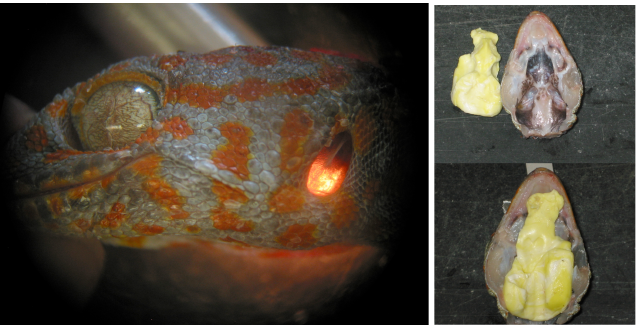
\includegraphics[width=.85\linewidth]{Diagrams/geckohead1.png}
       
      \footnotesize
      Tokay gecko with the head illuminated from the opposite side\footnote{Courtesy J.C. Dalsgaard (Syddansk Universitet)} (left) with mouth casts (right).
     \end{column}
  \end{columns}
\end{frame}

\subsection{Vibration Amplitude}
\begin{frame}[t]
\frametitle{Density Plot}
% \noindent Vibration Amplitude - $20\mathrm{Log}_{\mathrm{10}}\left| \dot{S}^0/\pi a^2_{\mathrm{cyl}}\right|$
\begin{variableblock}{}{bg= white,fg=black}{bg= white,fg=blue!75}
\begin{figure}[ht!]
 \centering 
 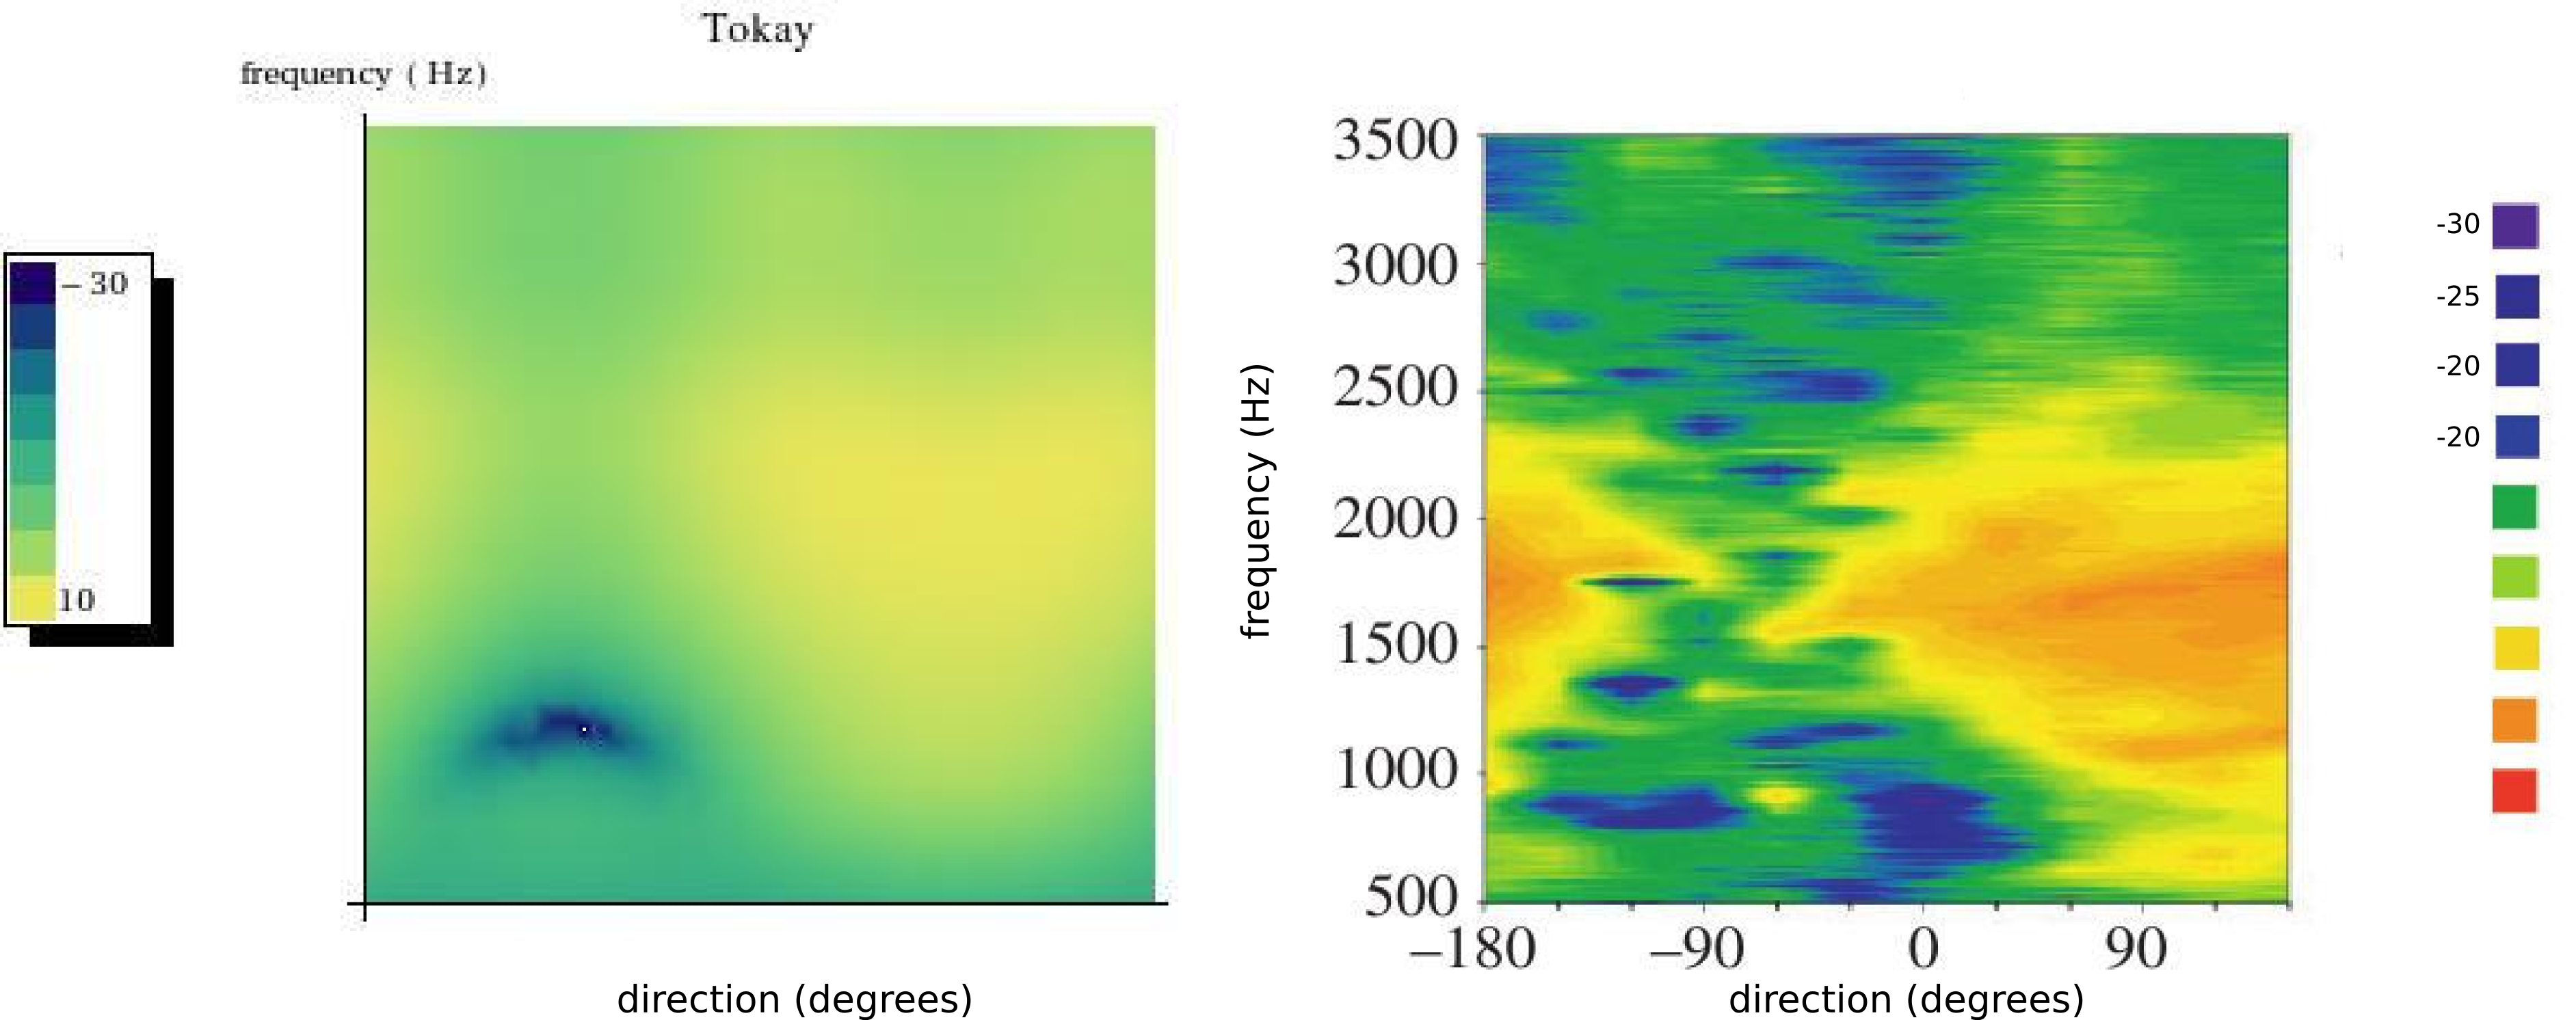
\includegraphics[width = 11 cm]{Diagrams/Plots/tokayvibampfull.png}
\end{figure}
\end{variableblock}
\begin{exampleblock}{}
\footnotesize
 \begin{itemize}
  \item Plot of vibration amplitude w.r.t direction \& frequency (Left: Calculated, Right: Experimental\footnote{\bibentry{dalsgaardmanley1}}).
  \item $\left|p_0\right|=\left|p_L\right|=1$ Pa.
 \end{itemize}
\end{exampleblock}
% \begin{columns}
%     \begin{column}{0.5\textwidth}
%       \centering
%       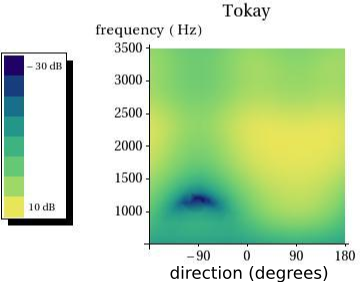
\includegraphics[width = 5.6 cm]{Diagrams/Presentation/tokayvibamp.png}\\
%      
%       \footnotesize \hspace{16pt} direction (degrees)
%     \end{column}
% 
%     \begin{column}{0.5\textwidth}
%     \textbf{}\\
%     %\textbf{}\\
%     \vspace{1pt}
%     \flushright
%       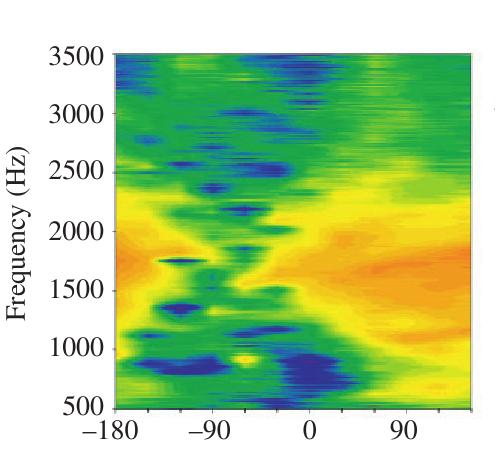
\includegraphics[width = 4.25 cm]{Diagrams/Presentation/tokayvibamp_exp.jpeg}\\
%       \centering
%       \footnotesize direction (degrees)
%     \end{column}
%   \end{columns}
\end{frame}

\begin{frame}[t]
\frametitle{Frequency Dependence}
%\noindent Frequency Dependence
\begin{variableblock}{}{bg= white,fg=black}{bg= white,fg=blue!75}
\begin{figure}[ht!]
 \centering 
 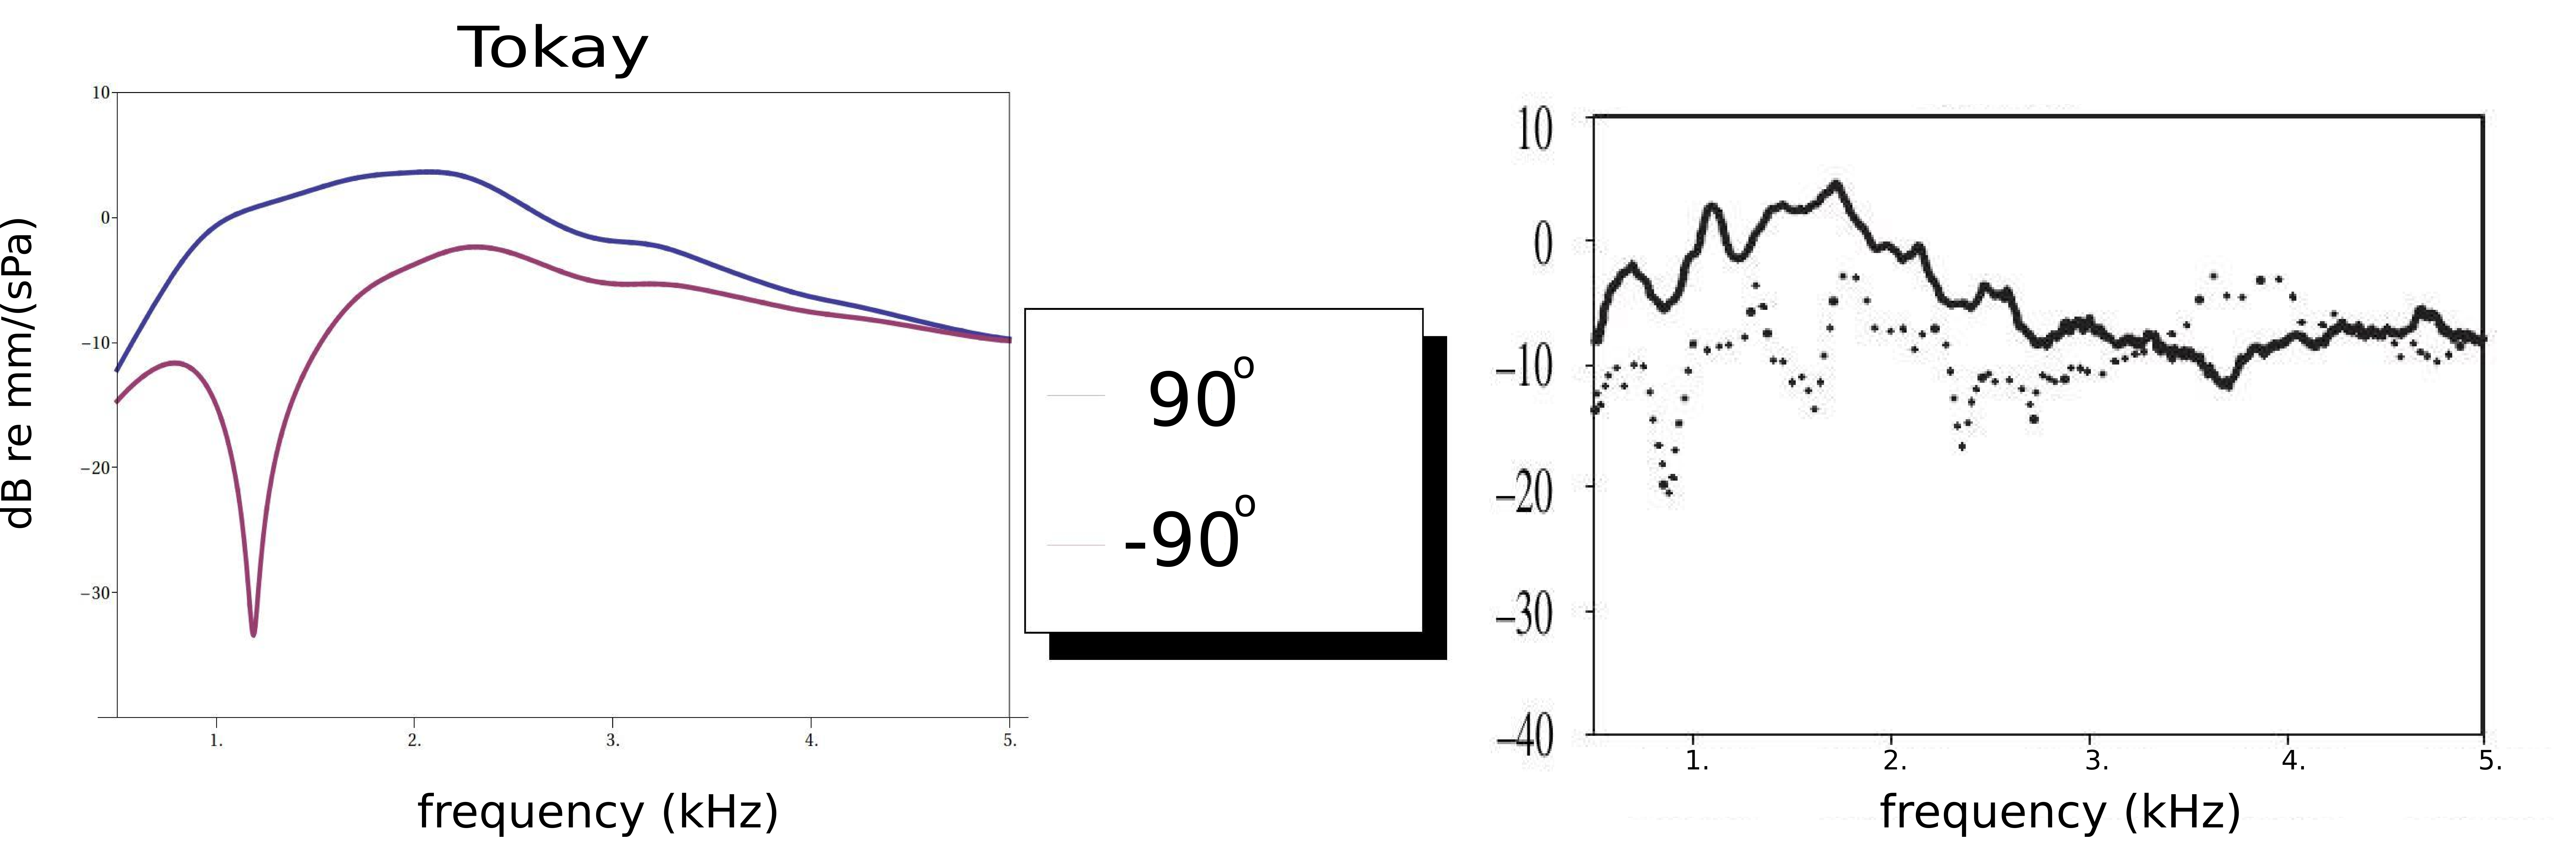
\includegraphics[width = 11 cm]{Diagrams/Presentation/tokayipsivscontrafull.png}
\end{figure}
\end{variableblock}
\begin{exampleblock}{}
\footnotesize
 \begin{itemize}
  \item Frequency dependence of $20\mathrm{Log}_{\mathrm{10}}\left| \dot{S}^0/\pi a^2_{\mathrm{cyl}}\right|$ for $\theta=90^\circ$. (Left:Calculated, Right:Experimental)
  \item $\left|p_0\right|=\left|p_L\right|=1$ Pa.
  \item Ipsilateral response $>$ Contralateral response.
 \end{itemize}
\end{exampleblock}
\end{frame}

\begin{frame}[t]
%\frametitle{Direction Dependence}
 \begin{columns}
     \begin{column}{0.45\textwidth}
     %\frametitle{Direction Dependence}
     \noindent \color{blue} Direction Dependence.
     \small
     \flushleft
\onslide<1>{\begin{exampleblock}{}
  \begin{itemize}
   \item Inputs to ears \begin{itemize}
			  \footnotesize
                         \item Negligible level (amplitude) difference
                         \item Small time (phase) difference
                        \end{itemize}
   \item Response is highly directional.

  \end{itemize}
 \end{exampleblock}}

 \vfill
 \onslide<2>{\begin{variableblock}{}{bg= blue!5,fg=black}{bg= blue!5,fg=blue!75}
	      \begin{itemize}
	       \item Independent vibration amplitudes not enough.
               \item Localization requires using information from both ears.
               \end{itemize}
              \end{variableblock}}
              \end{column}
              
              \begin{column}{0.55\textwidth}
  \only<1>{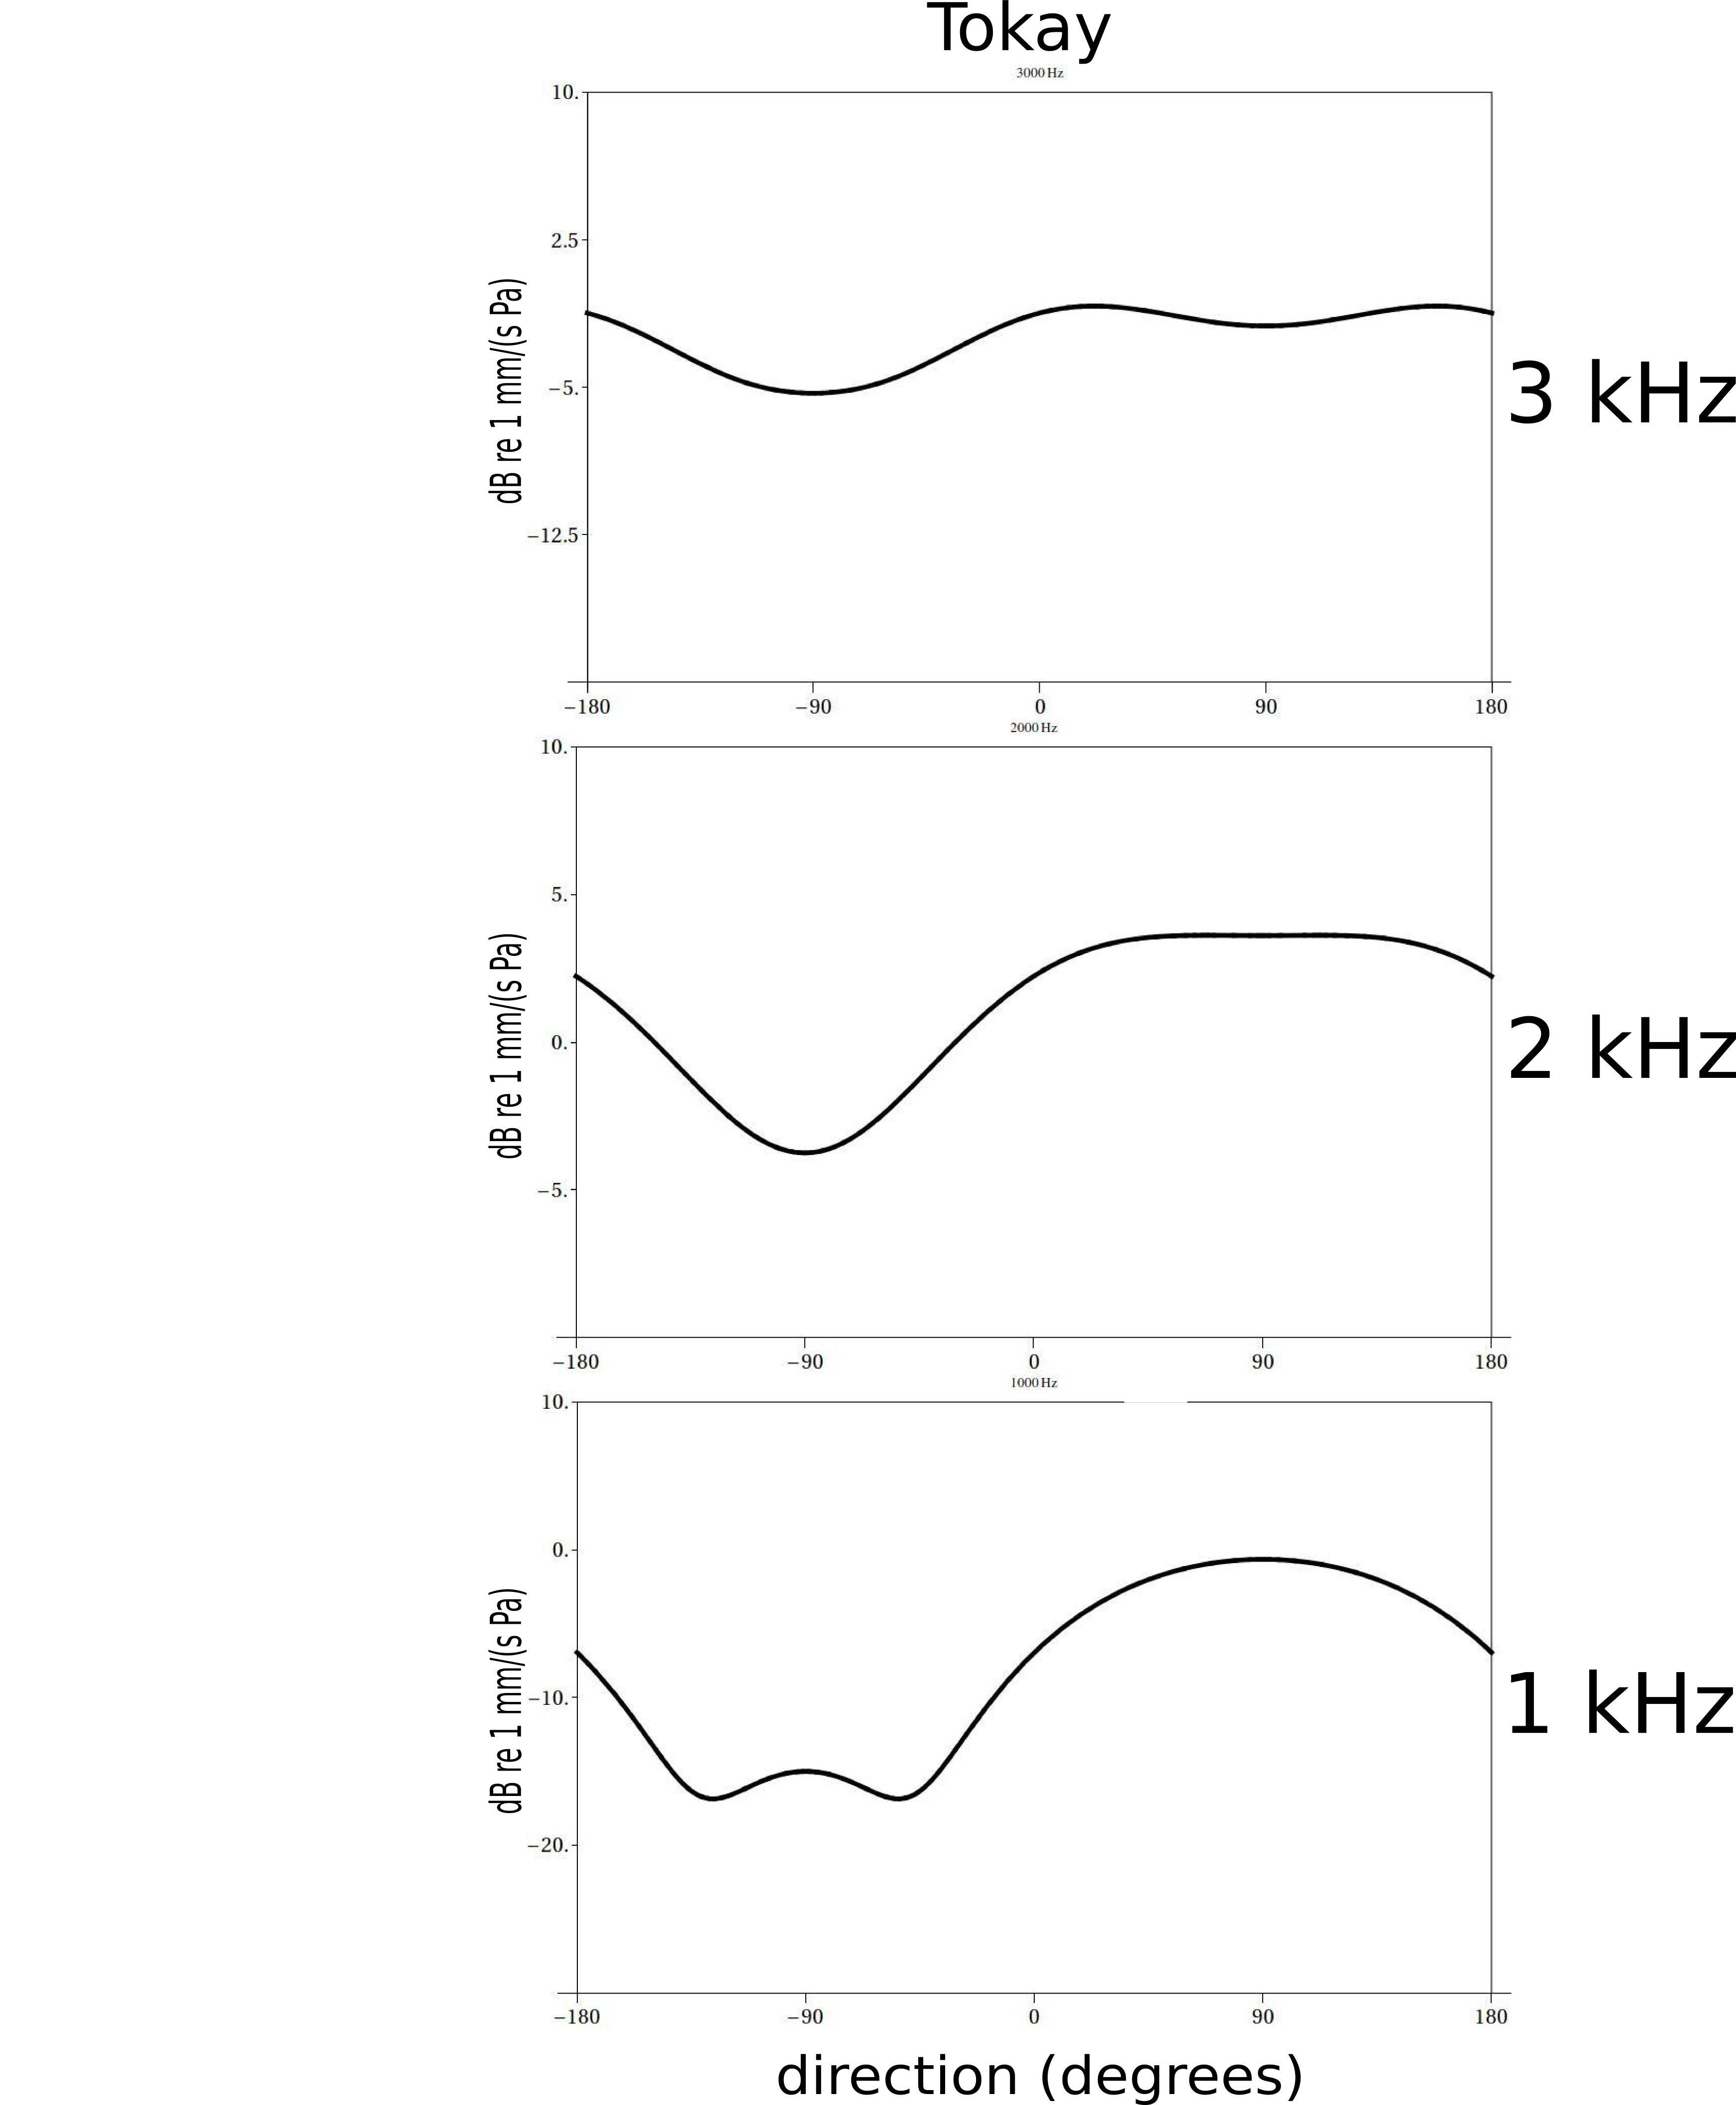
\includegraphics[width = 6.2 cm]{Diagrams/Presentation/directionplots.png}}
  %  \only<2>{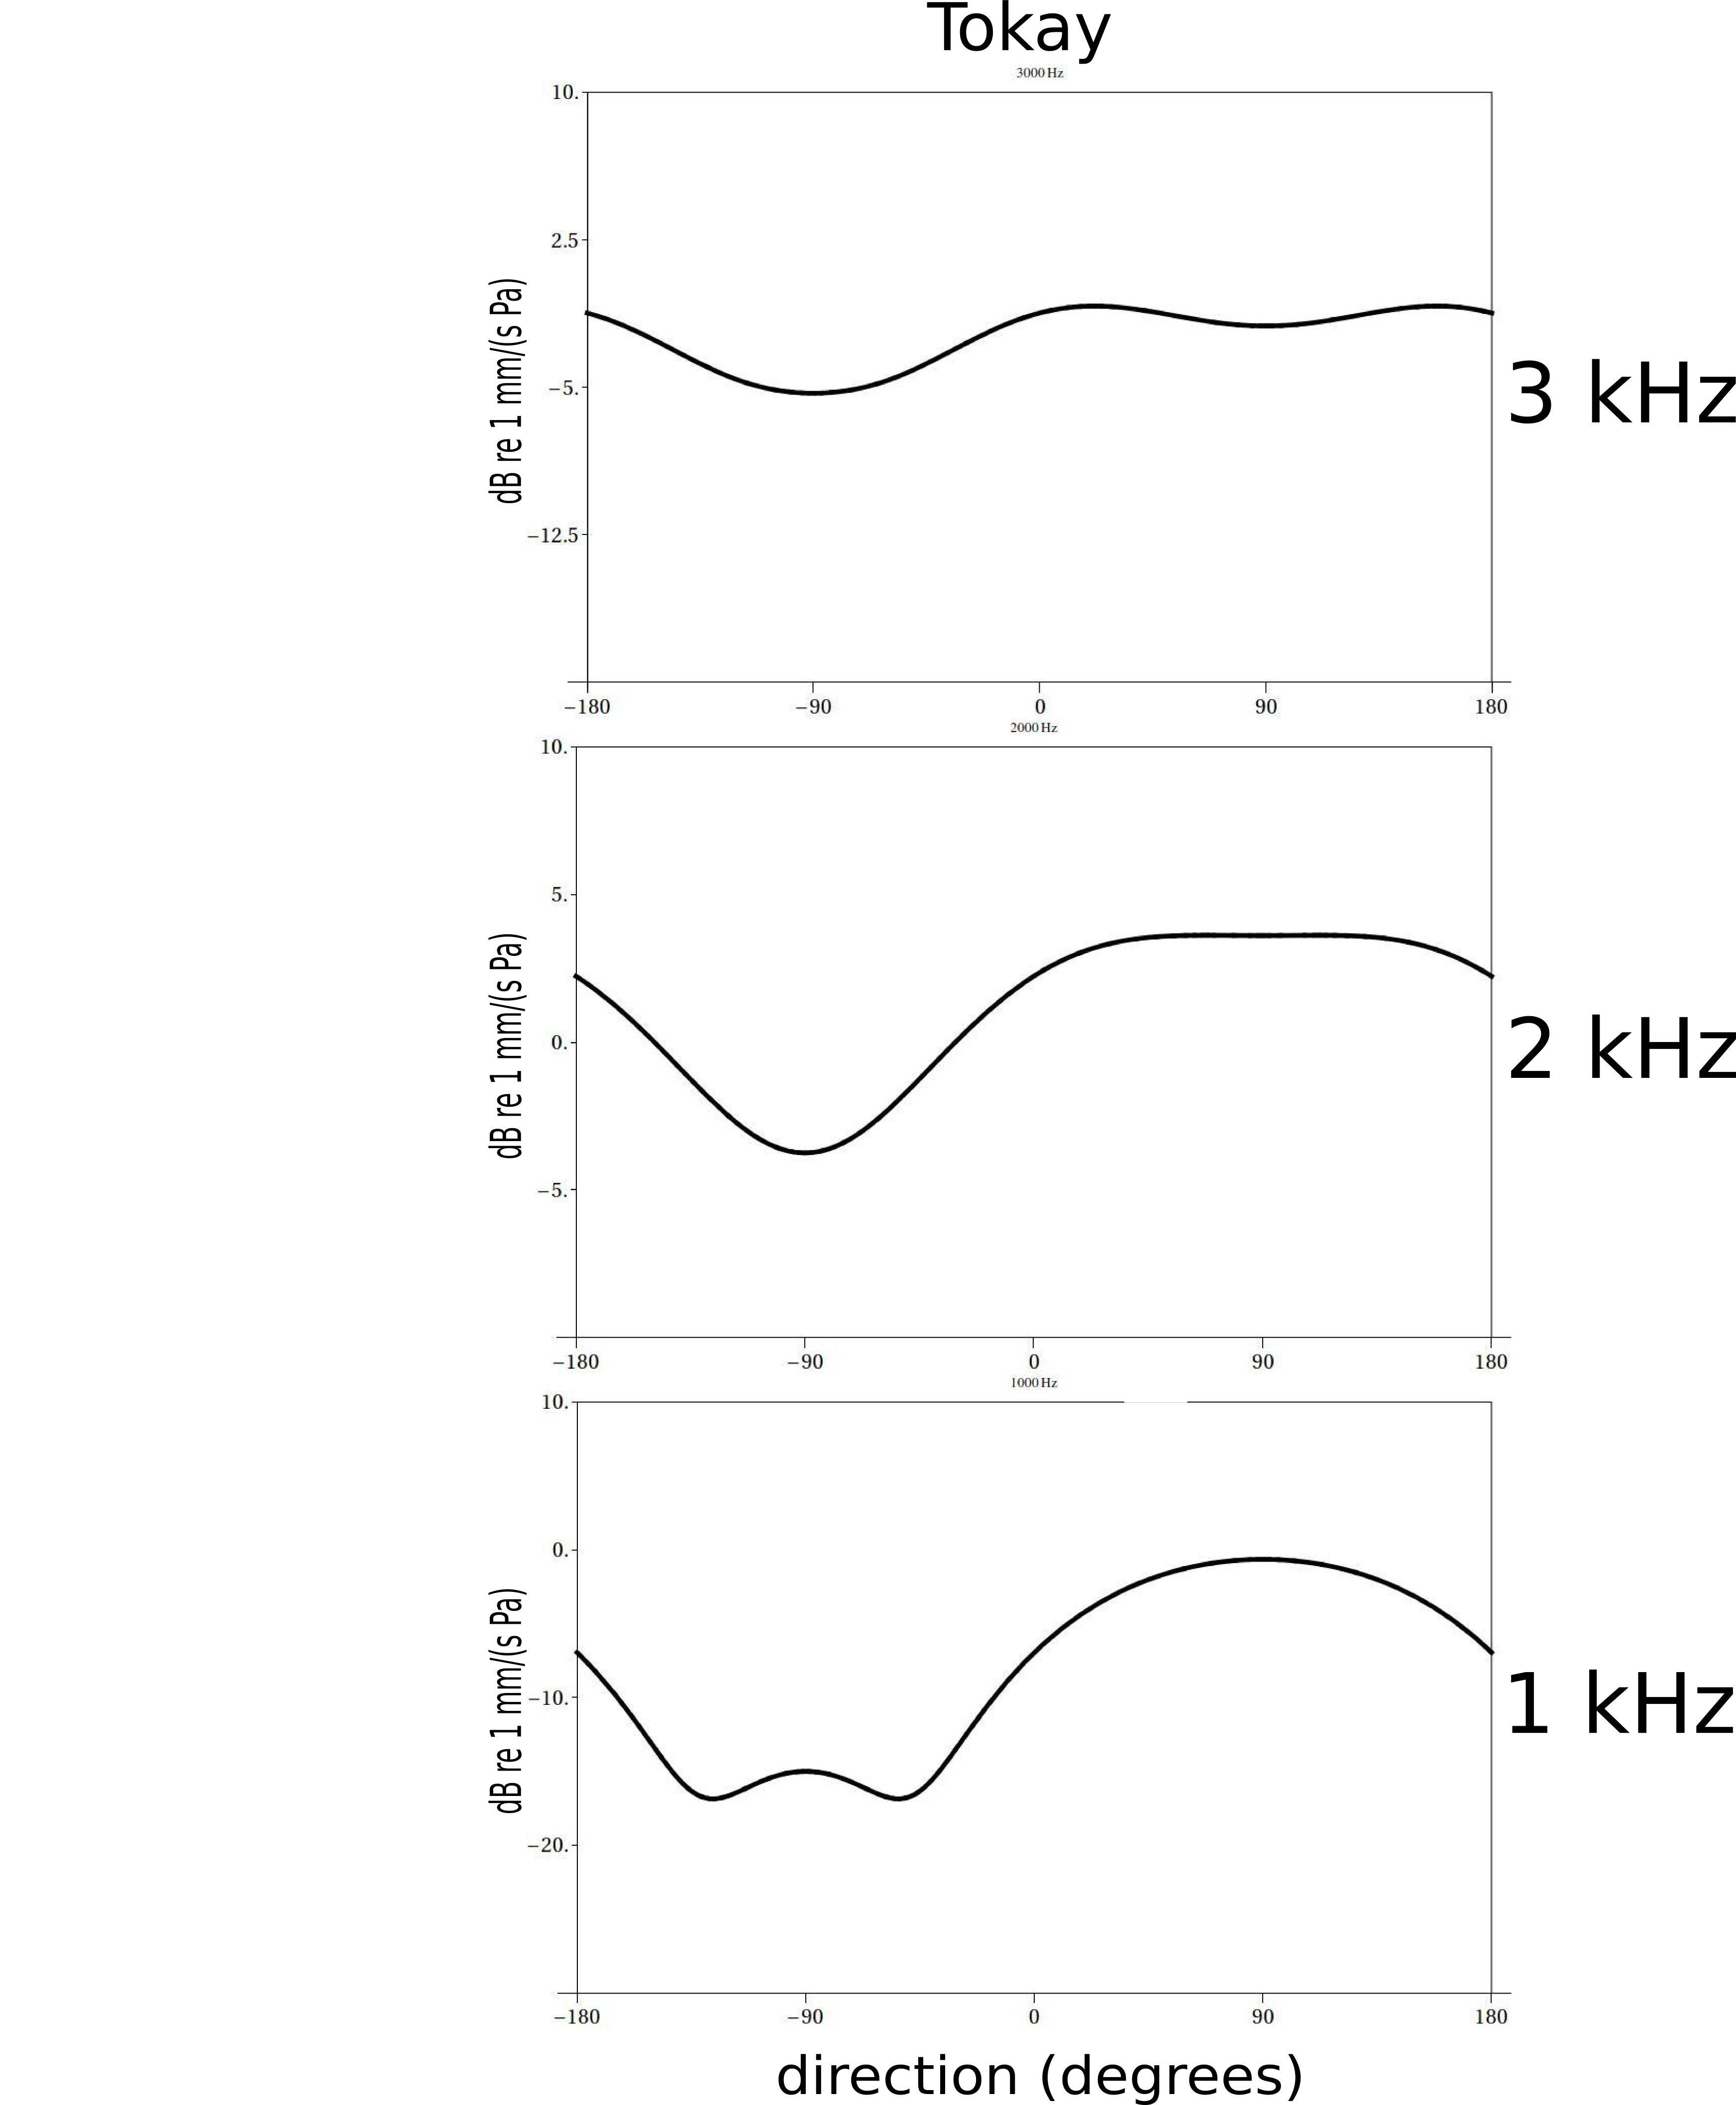
\includegraphics[width = 6.2 cm]{Diagrams/Presentation/directionplots.png}}
  \only<2>{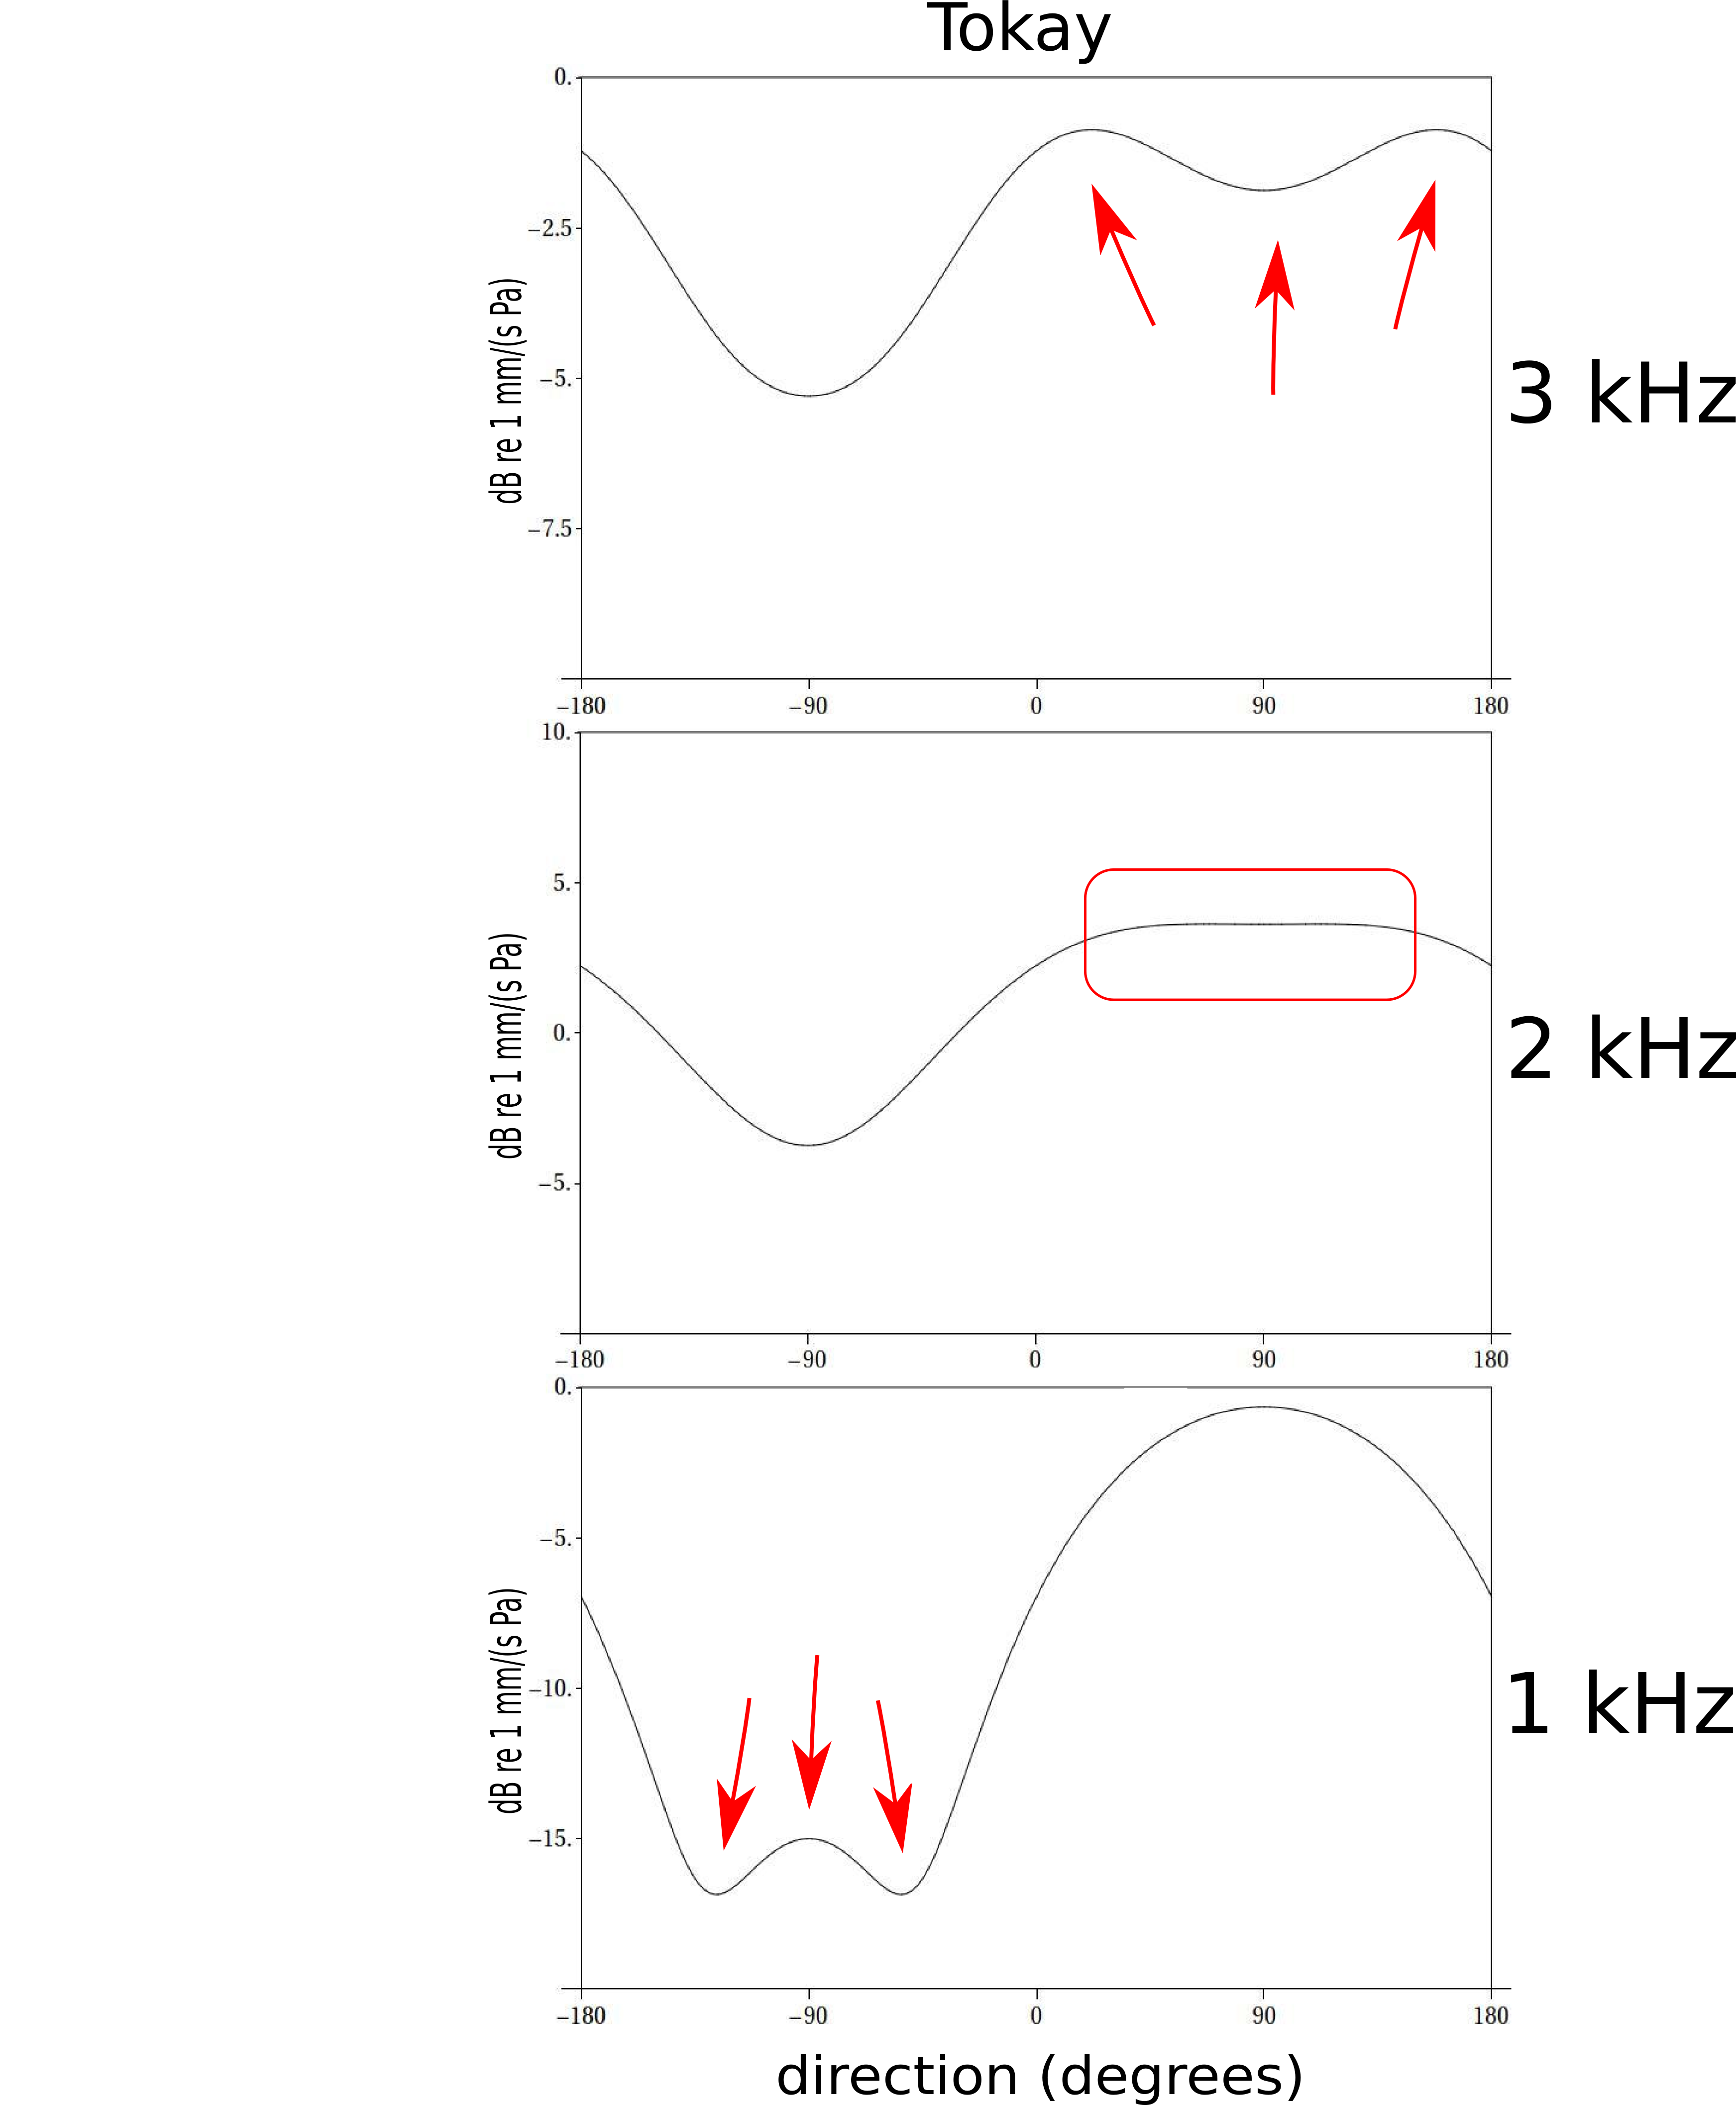
\includegraphics[width = 6.2 cm]{Diagrams/Presentation/directionplots2.png}}
\end{column}
   \end{columns}



\end{frame}
\subsection{Directional Cues}

\begin{frame}[t]
\frametitle{Hearing Cues}
 \begin{columns}
     \begin{column}{0.5\textwidth}
 \begin{variableblock}{}{bg= blue!5,fg=black}{bg= blue!5,fg=blue!75}
\onslide<1->{Internal Level Difference (iLD) - 
\begin{equation}
  \mbox{iLD}\vcentcolon= 20\mbox{Log}_{10}\left|\frac{\dot{S}^0}{\dot{S}^L}\right|\label{iLDfirstdef}
\end{equation}}
\onslide<2->{Internal Time Difference (iTD) - 
\begin{equation}
 \mbox{iTD}\vcentcolon= \mbox{Arg}\left(\frac{\dot{S}^0}{\dot{S}^L}\right)/\omega\label{iTDfirstdef}
\end{equation}}
\end{variableblock}
\end{column}
\begin{column}{0.5\textwidth}
\onslide<3->{\begin{exampleblock}{Requirements}
 \begin{enumerate}
 \small
 \item \label{listitem1} Both increase with the adjacency of the sound source. Max at $\theta=90^\circ$ and min at $\theta=-90^\circ$.
 \item \label{listitem3} Both vanish at $\theta=0^\circ,\ \pm 180^\circ$.
 \item \label{listitem2} iTD $\approx$ constant for a given frequency range. Advantageous for neuronal processing. 
\end{enumerate}
\end{exampleblock}}
\end{column}
\end{columns}

\end{frame}


\subsubsection{Internal Level Difference}
\begin{frame}[t]
\frametitle{iLD Density Plot}
%\noindent Internal Level Difference

     \begin{variableblock}{}{bg= white,fg=black}{bg= white,fg=blue!75}
 \begin{figure}[ht!]
 \centering 
 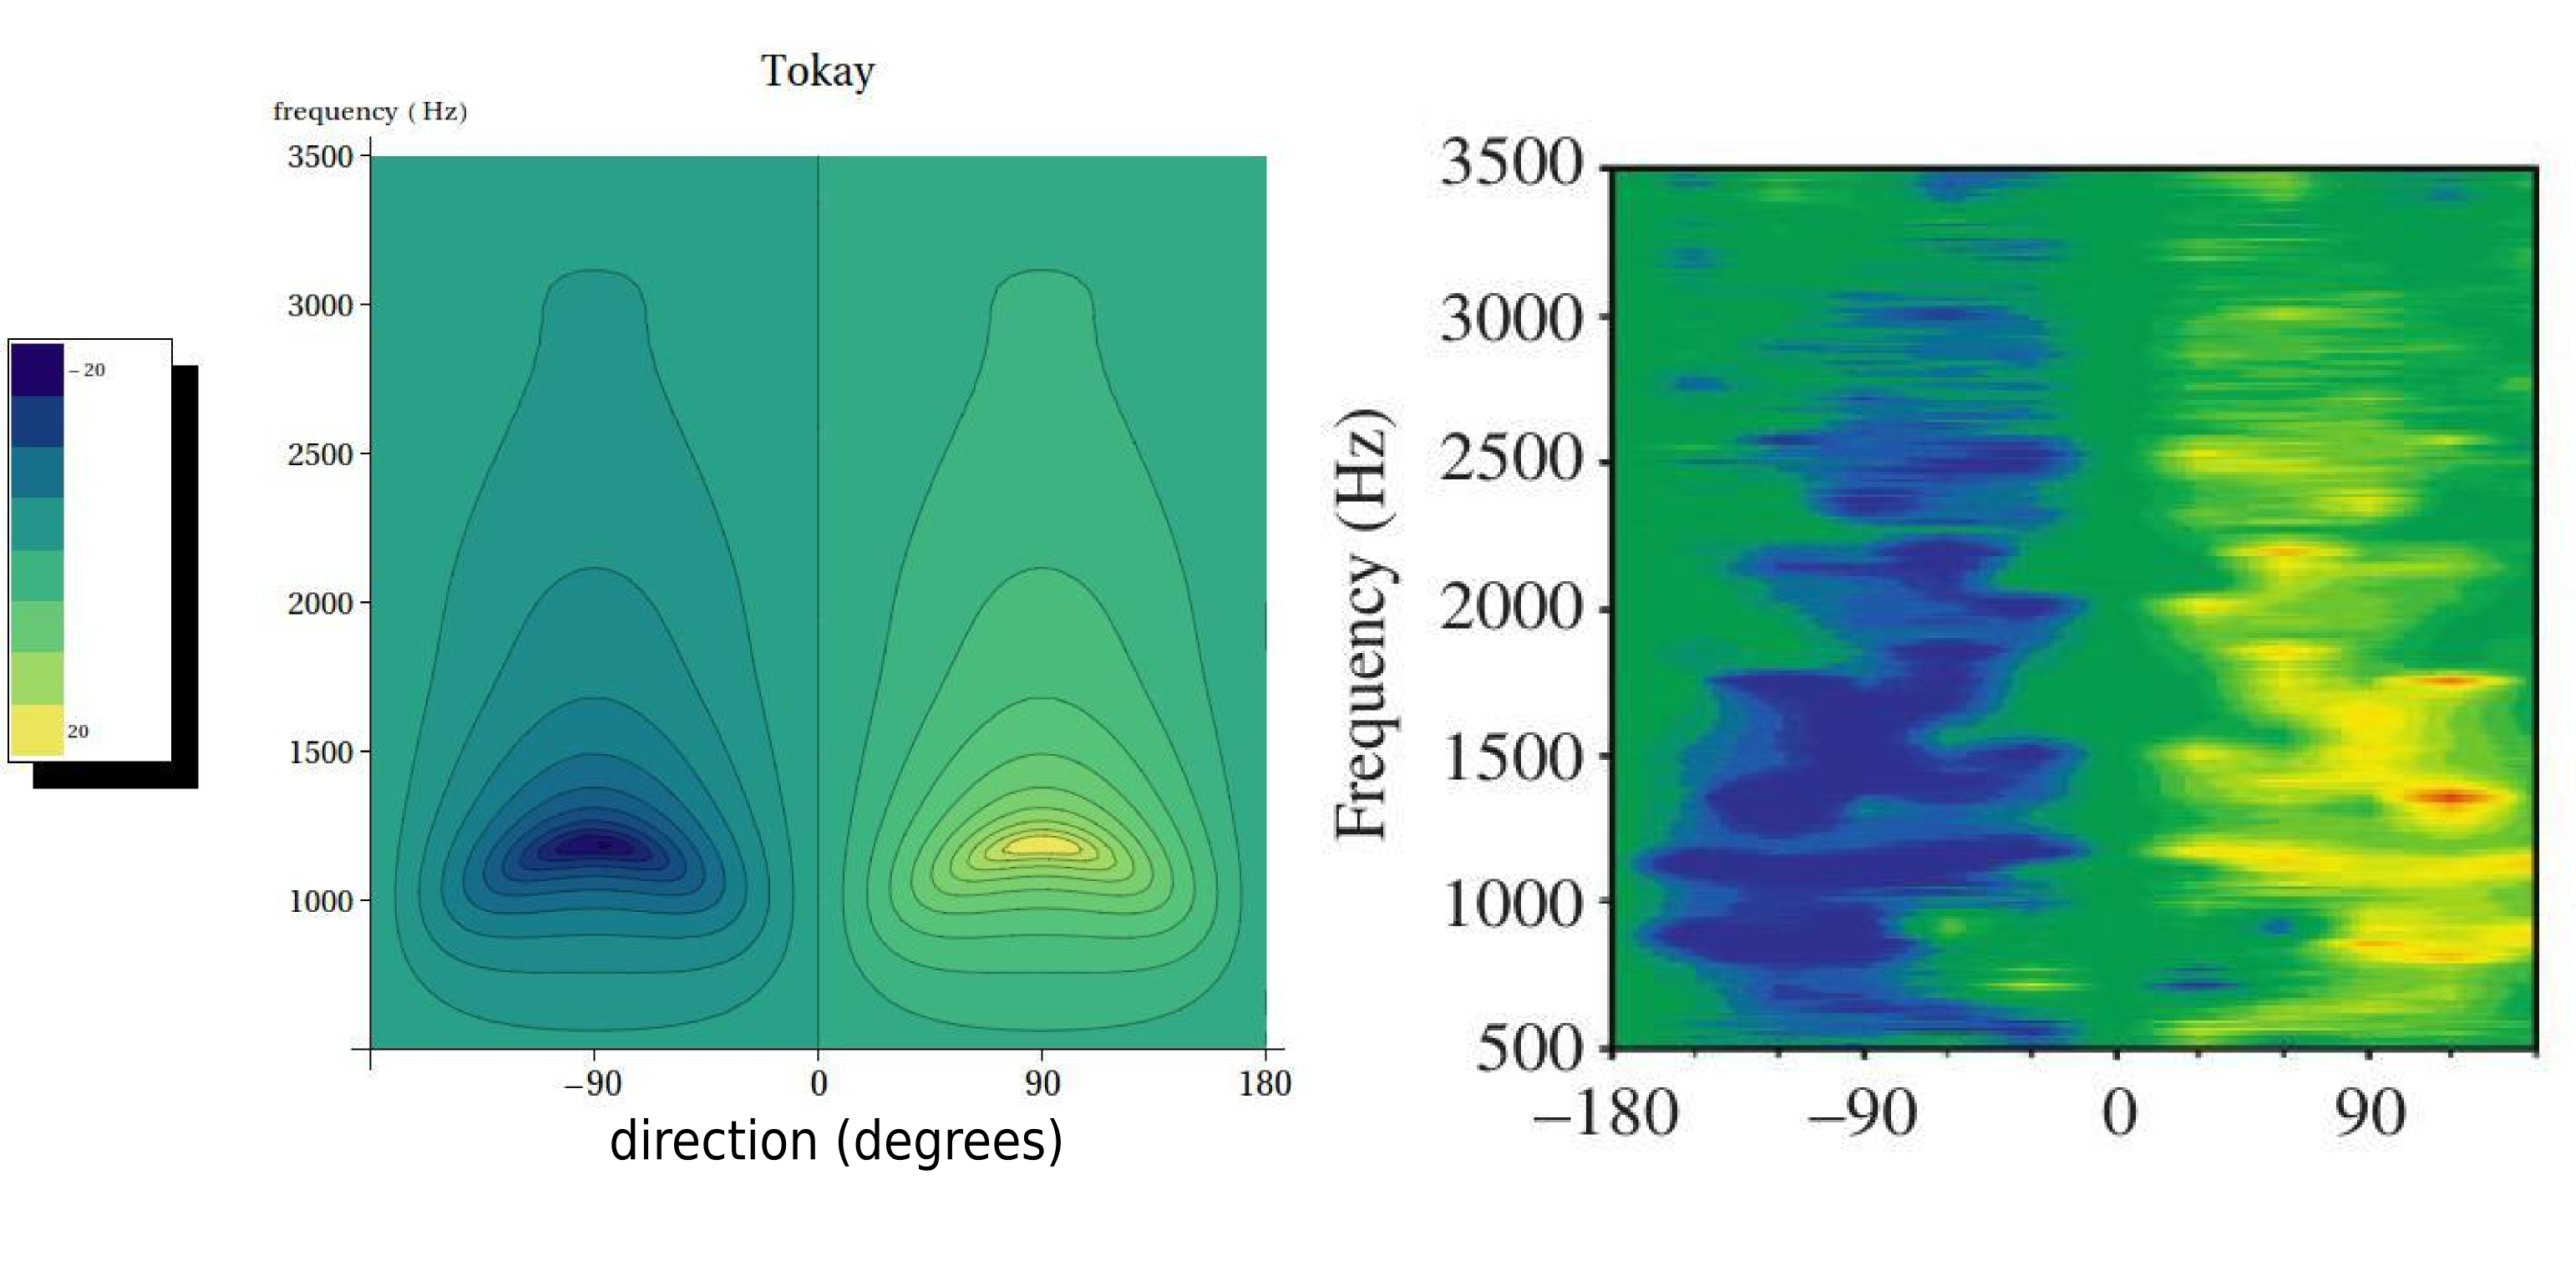
\includegraphics[width = 11 cm]{Diagrams/Plots/iLD/tokayiLDboth.png}
\end{figure}
\end{variableblock}


\begin{exampleblock}{}
\footnotesize
 \begin{itemize}
  \item Plot of iLD, against frequency and direction.
  \item Left: Calculated, Right: Experimental
 \end{itemize}
\end{exampleblock}
\end{frame}

\begin{frame}[t]
\frametitle{iLD Frequency/Direction Dependence}
%\noindent iLD Spectrum and Direction Dependence
\begin{columns}
\begin{column}{0.5\textwidth}
 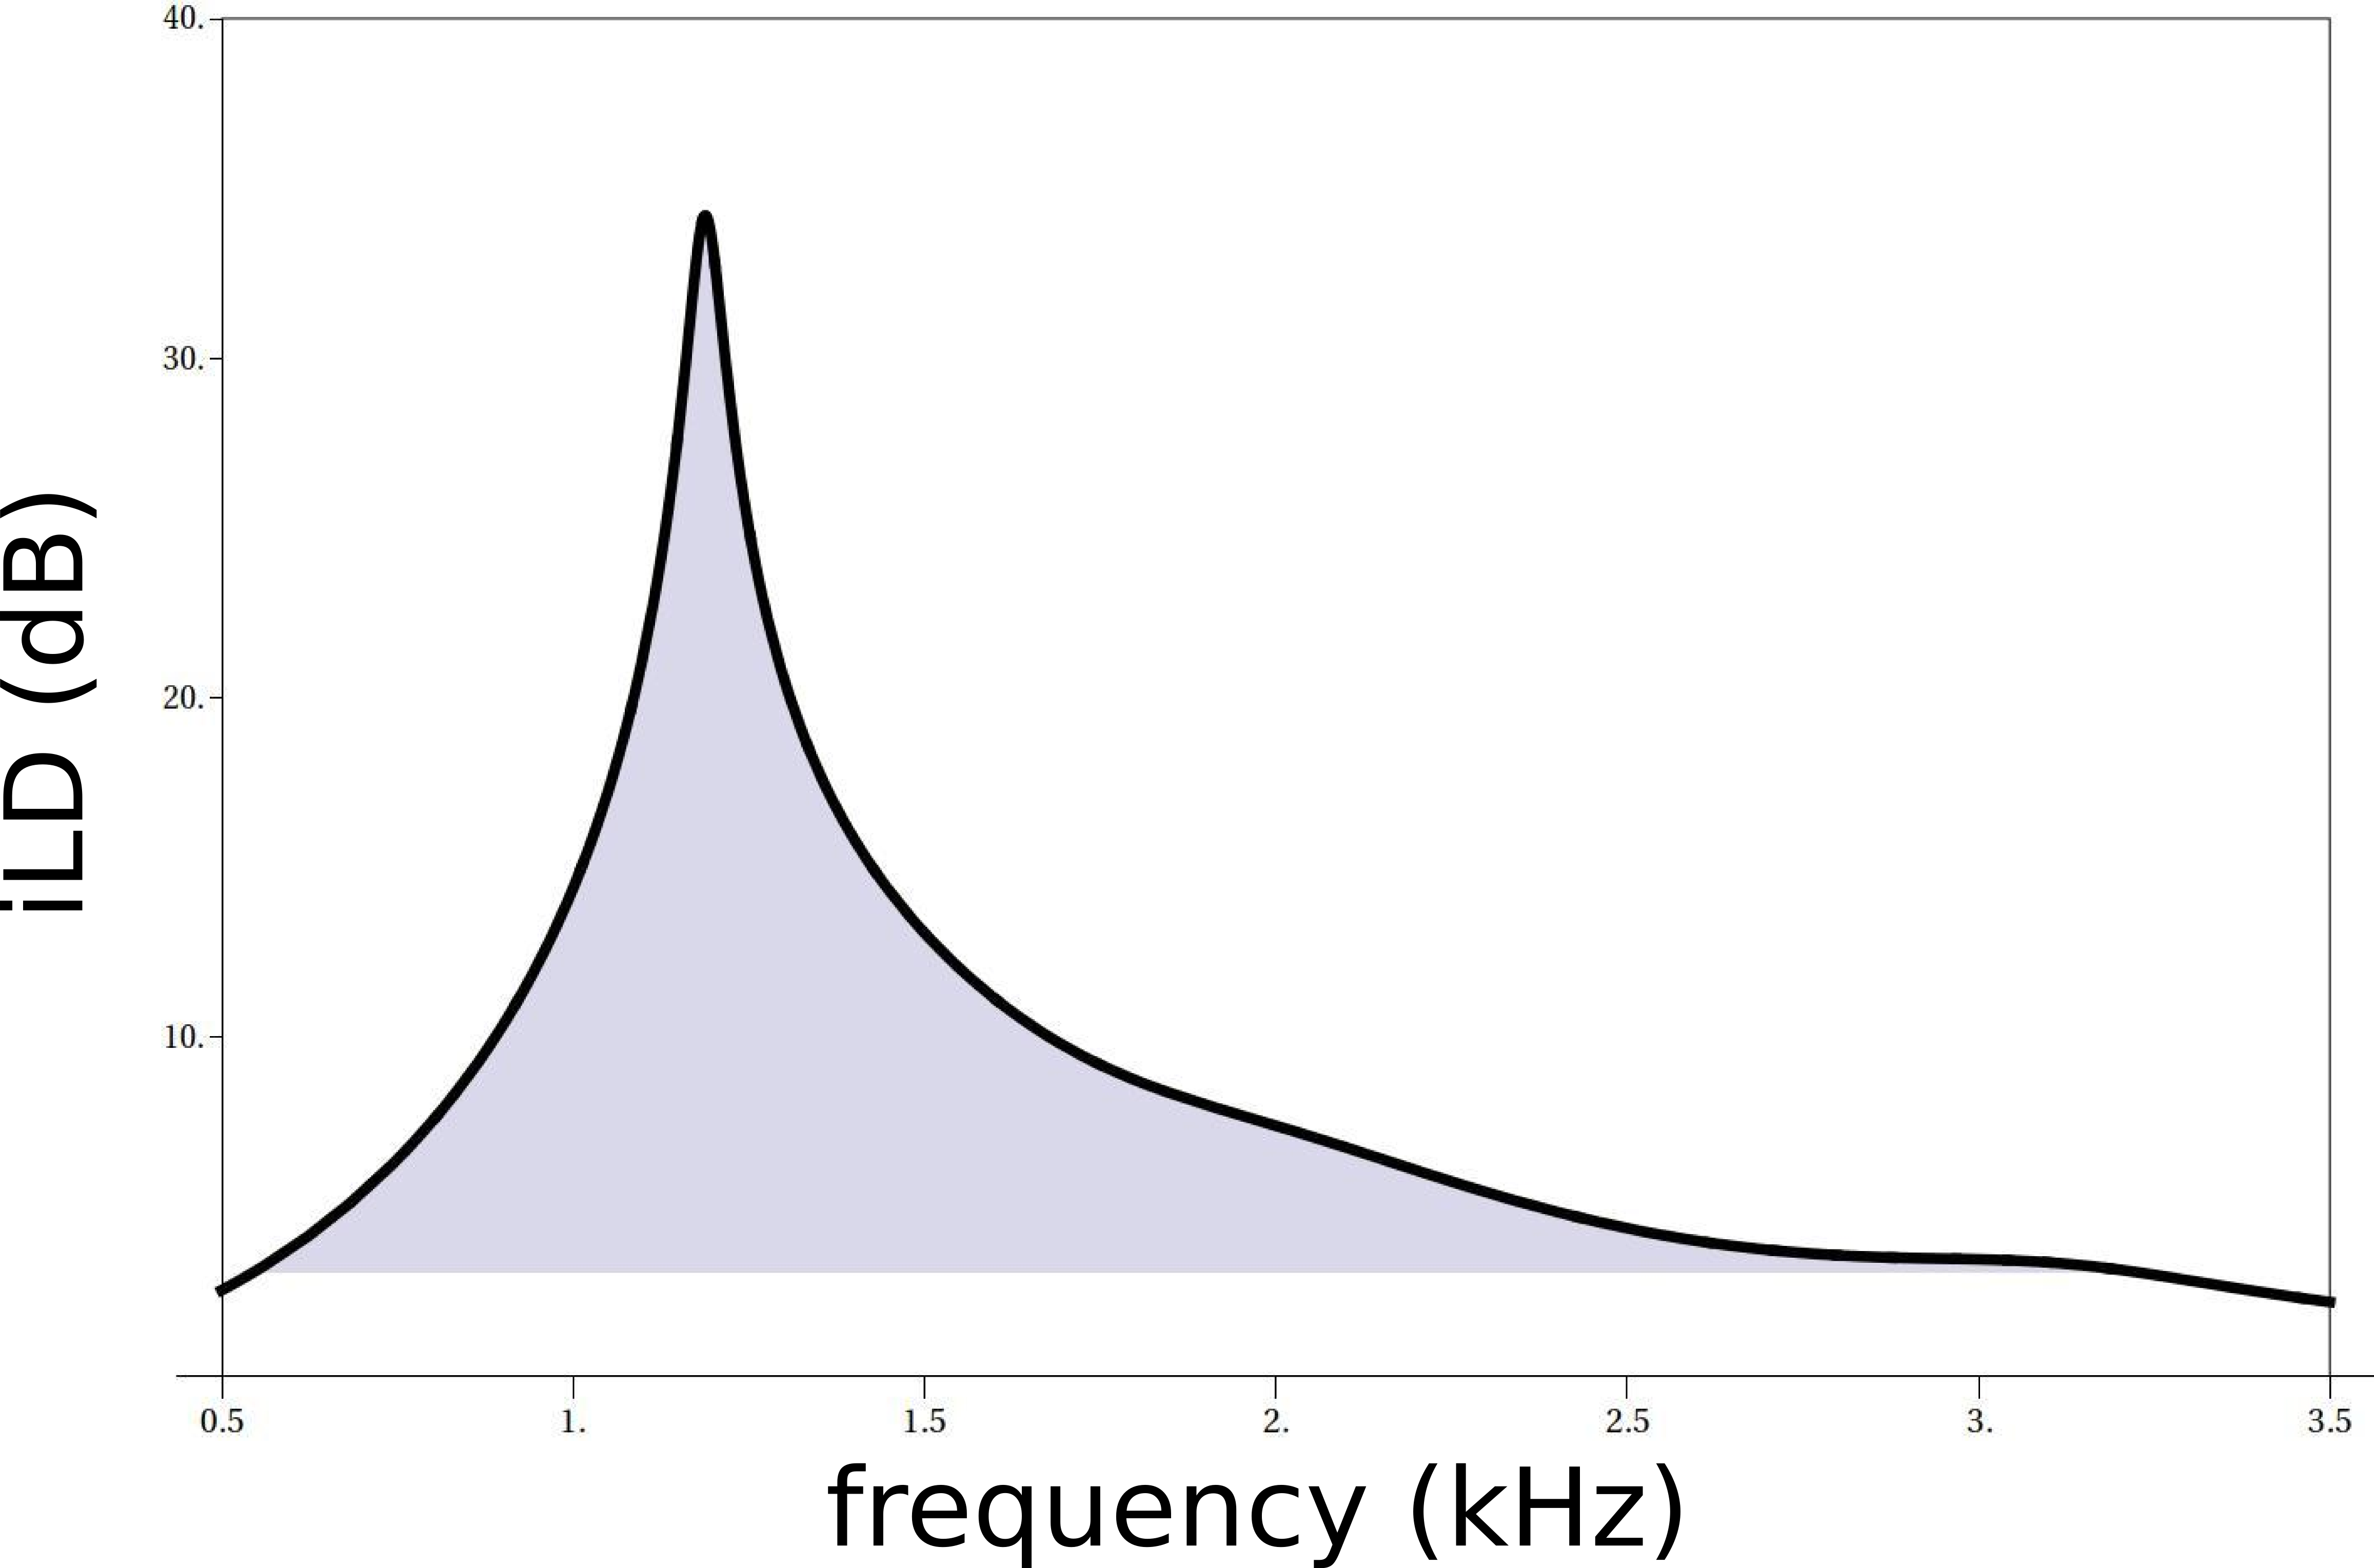
\includegraphics[width = 6 cm]{Diagrams/Presentation/iLDspectrum.png}
\begin{exampleblock}{}
\small
 \begin{itemize}
  \item iLD is a better cue at higher frequencies.
  \item Peak response at $\sim f_0$.
 \end{itemize}
\end{exampleblock}
\end{column}
     \begin{column}{0.5\textwidth}
     \flushright
 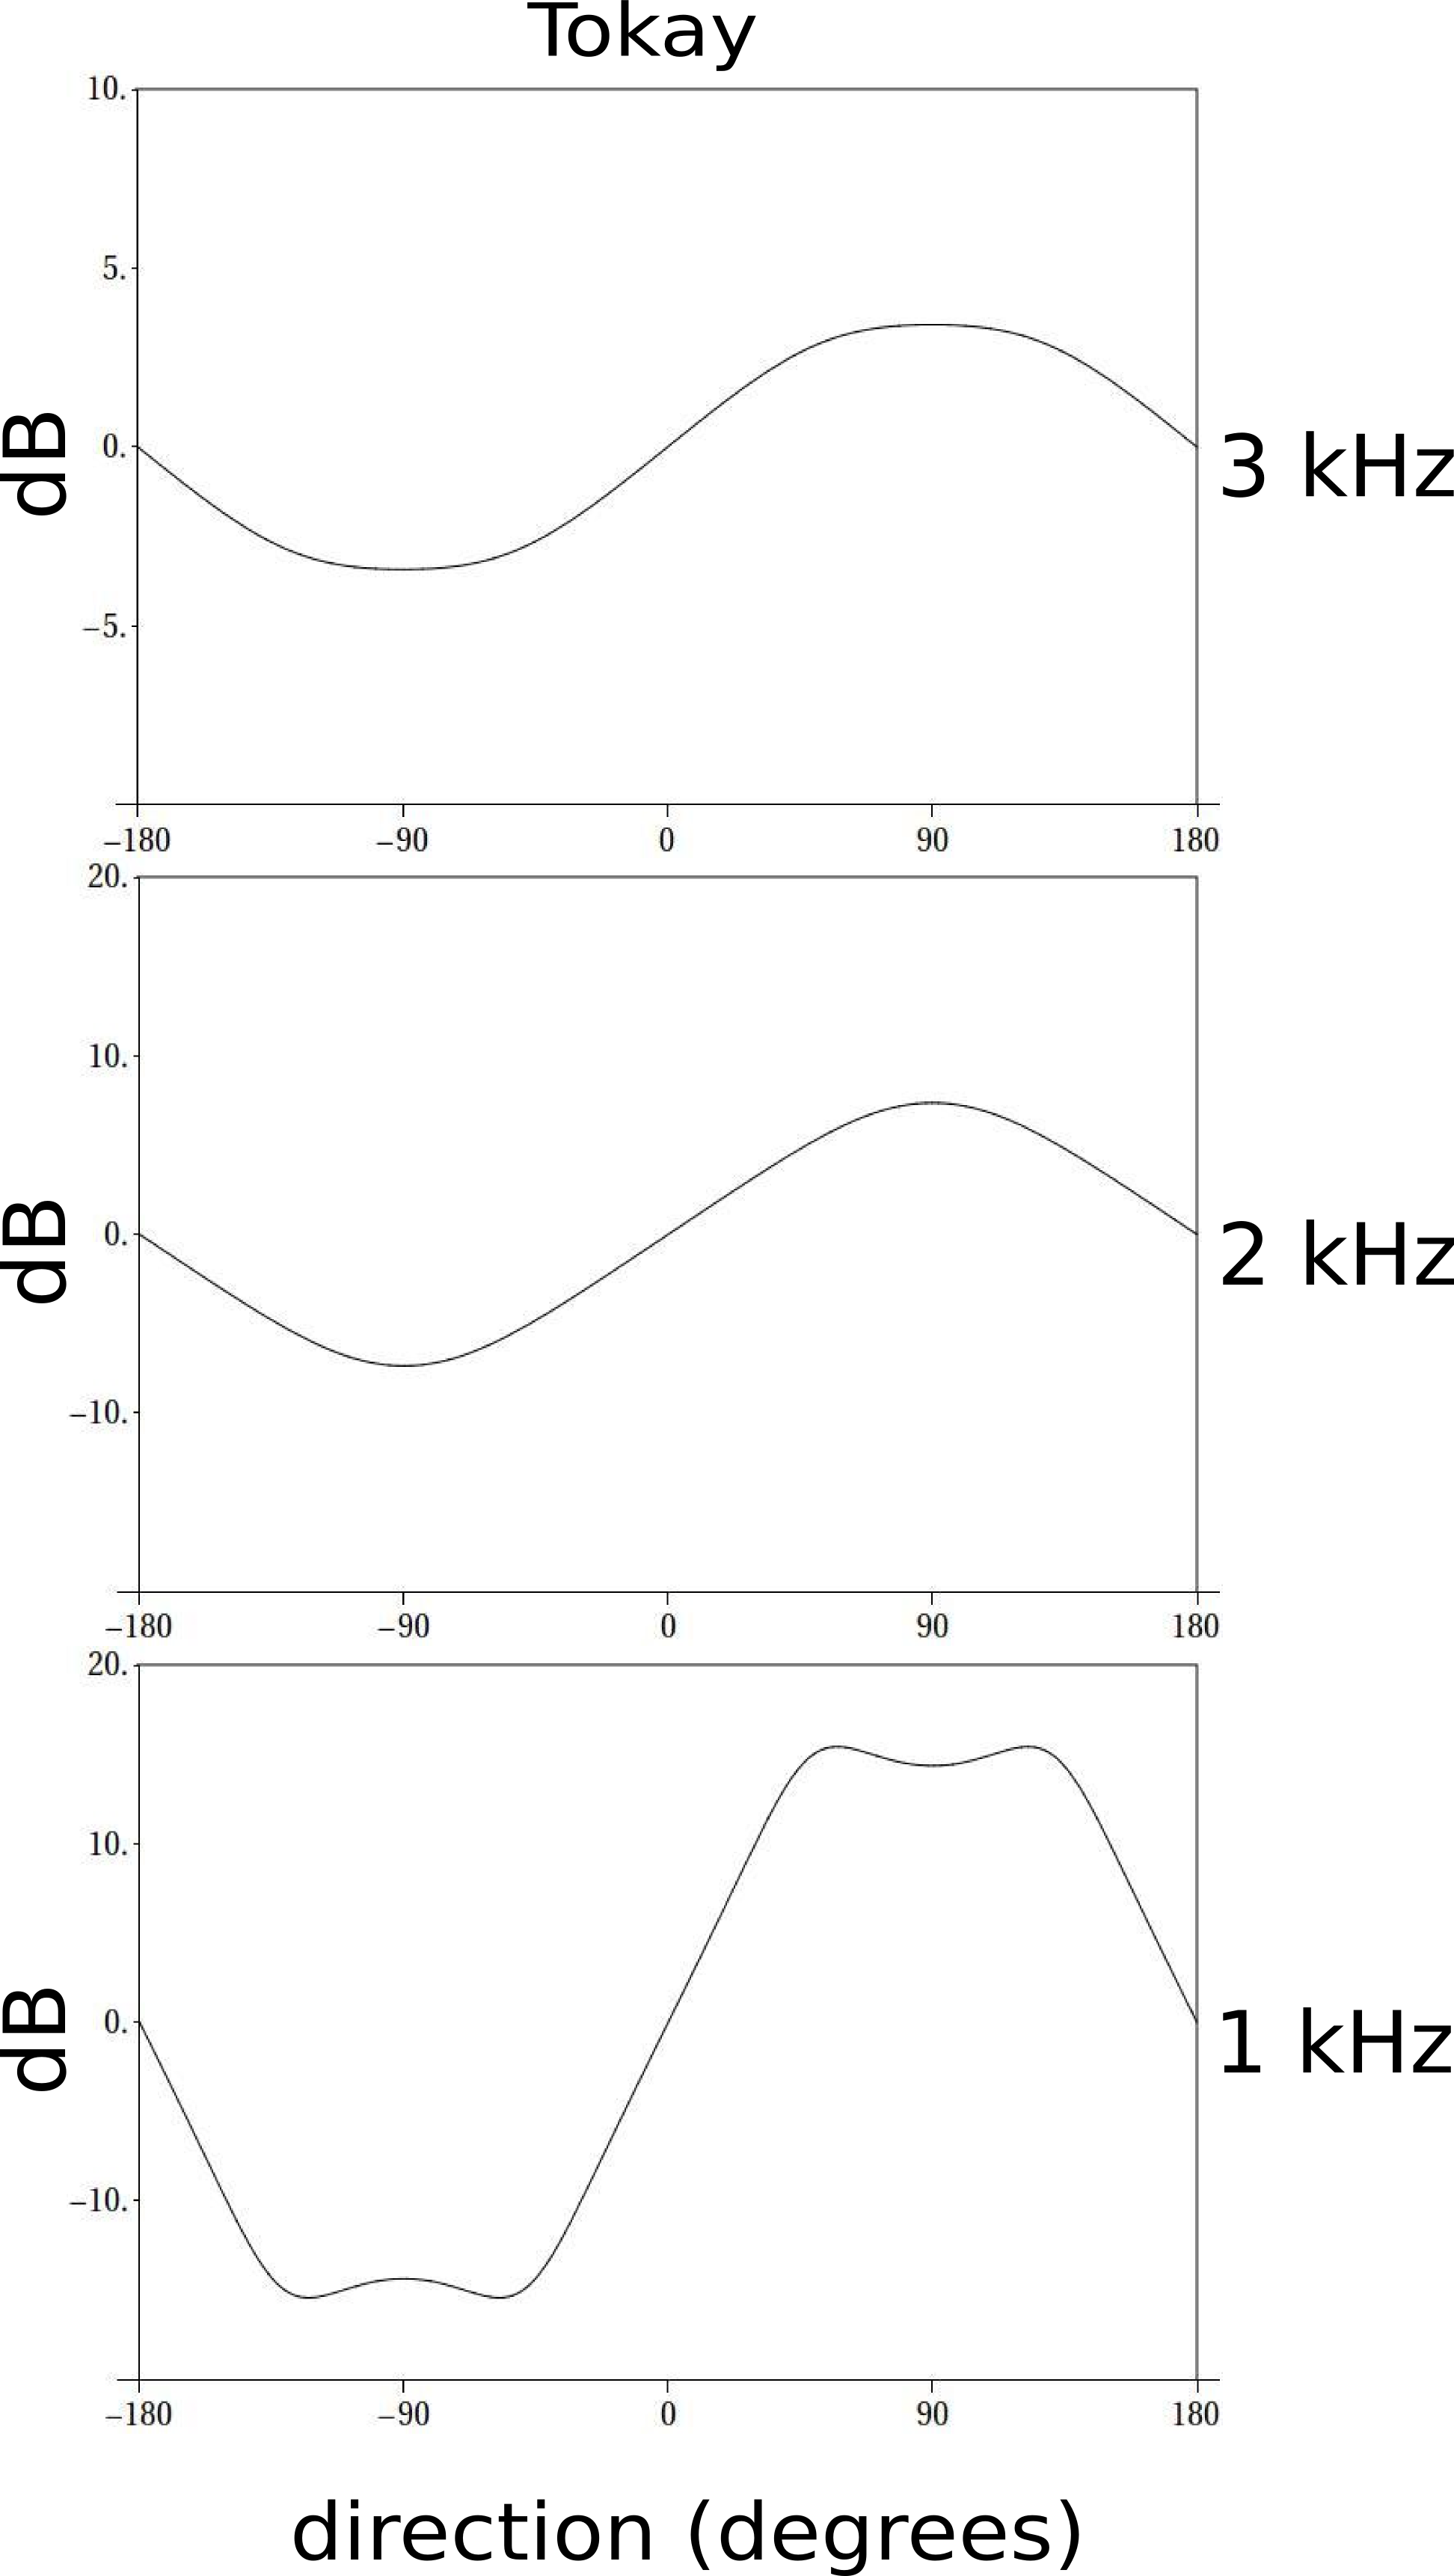
\includegraphics[width = 3.6 cm]{Diagrams/Presentation/iLDdirection.png}
\end{column}
\end{columns}
\end{frame}

\subsubsection{Internal Time Difference}
\begin{frame}[t]
\frametitle{iTD Frequency/Direction Dependence}
%\noindent iTD Spectrum and Direction Dependence
\begin{columns}
\begin{column}{0.5\textwidth}
 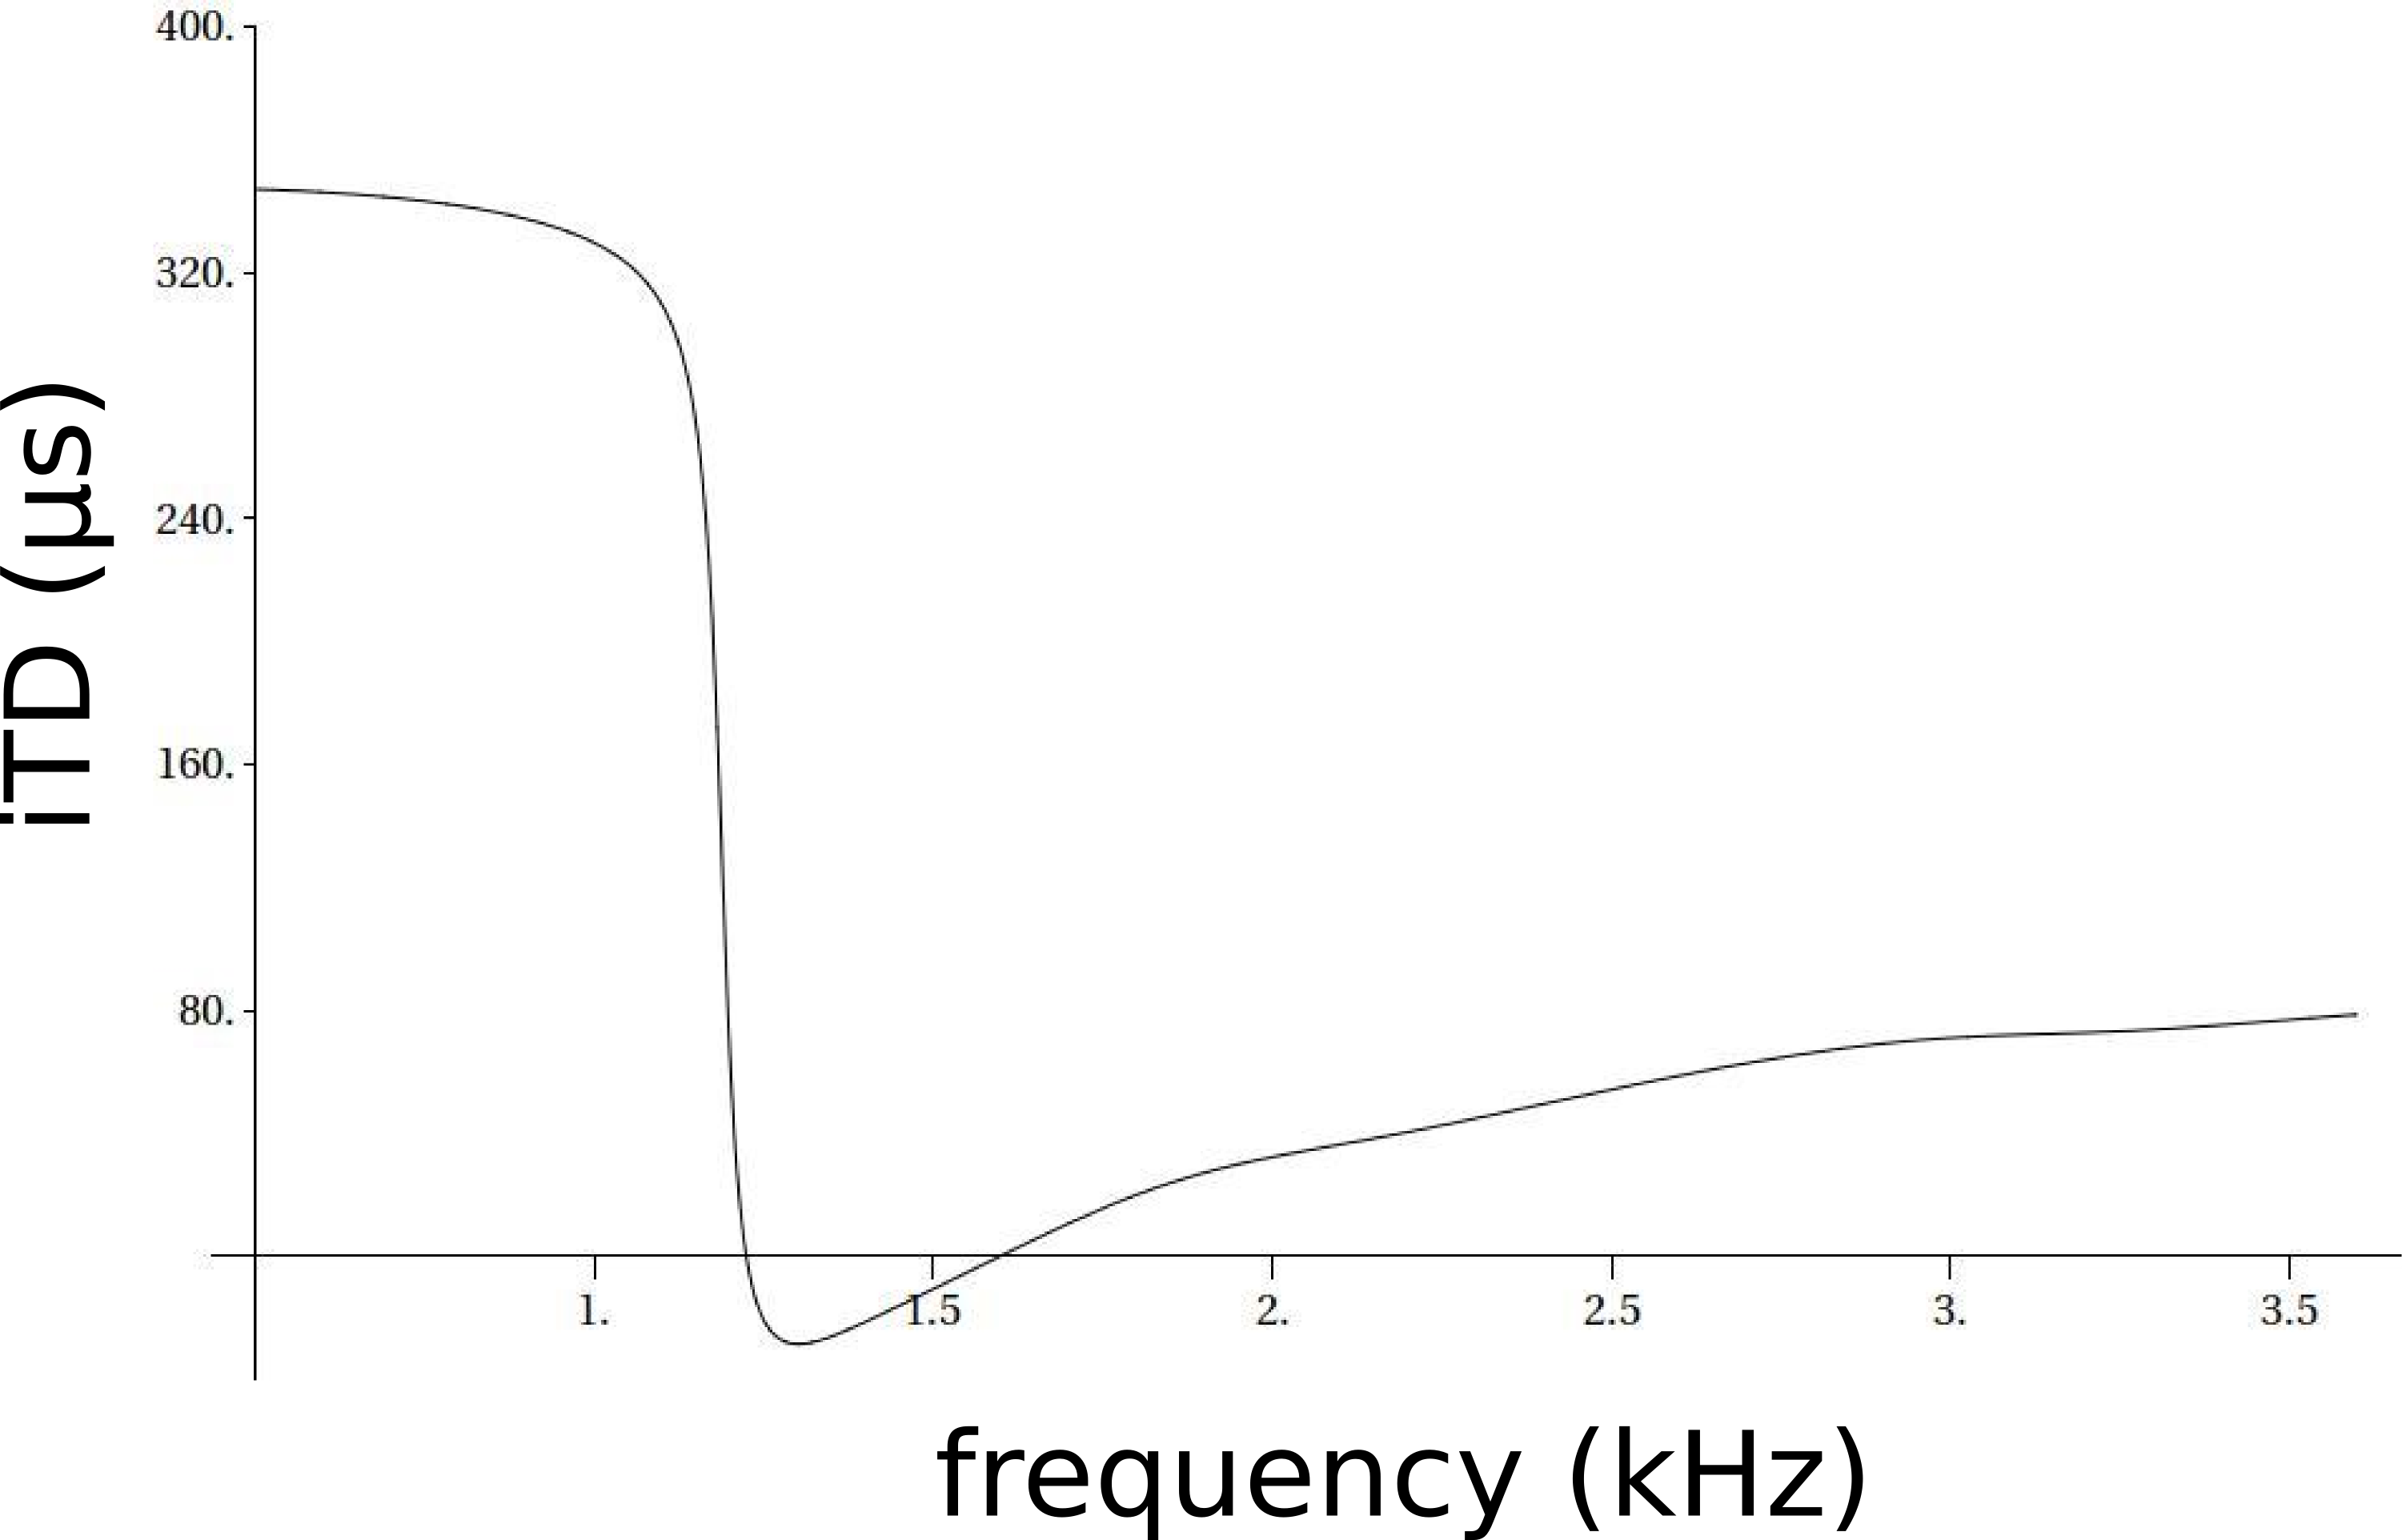
\includegraphics[width = 6 cm]{Diagrams/Presentation/iTDspectrum.png}
\begin{exampleblock}{}
\small
 \begin{itemize}
  \item iTD is a better cue at lower frequencies.
  \item constant upto $\sim f_0$.
  \item iTD $\approx$ 3ITD
 \end{itemize}
\end{exampleblock}
\end{column}
     \begin{column}{0.5\textwidth}
     \flushright
 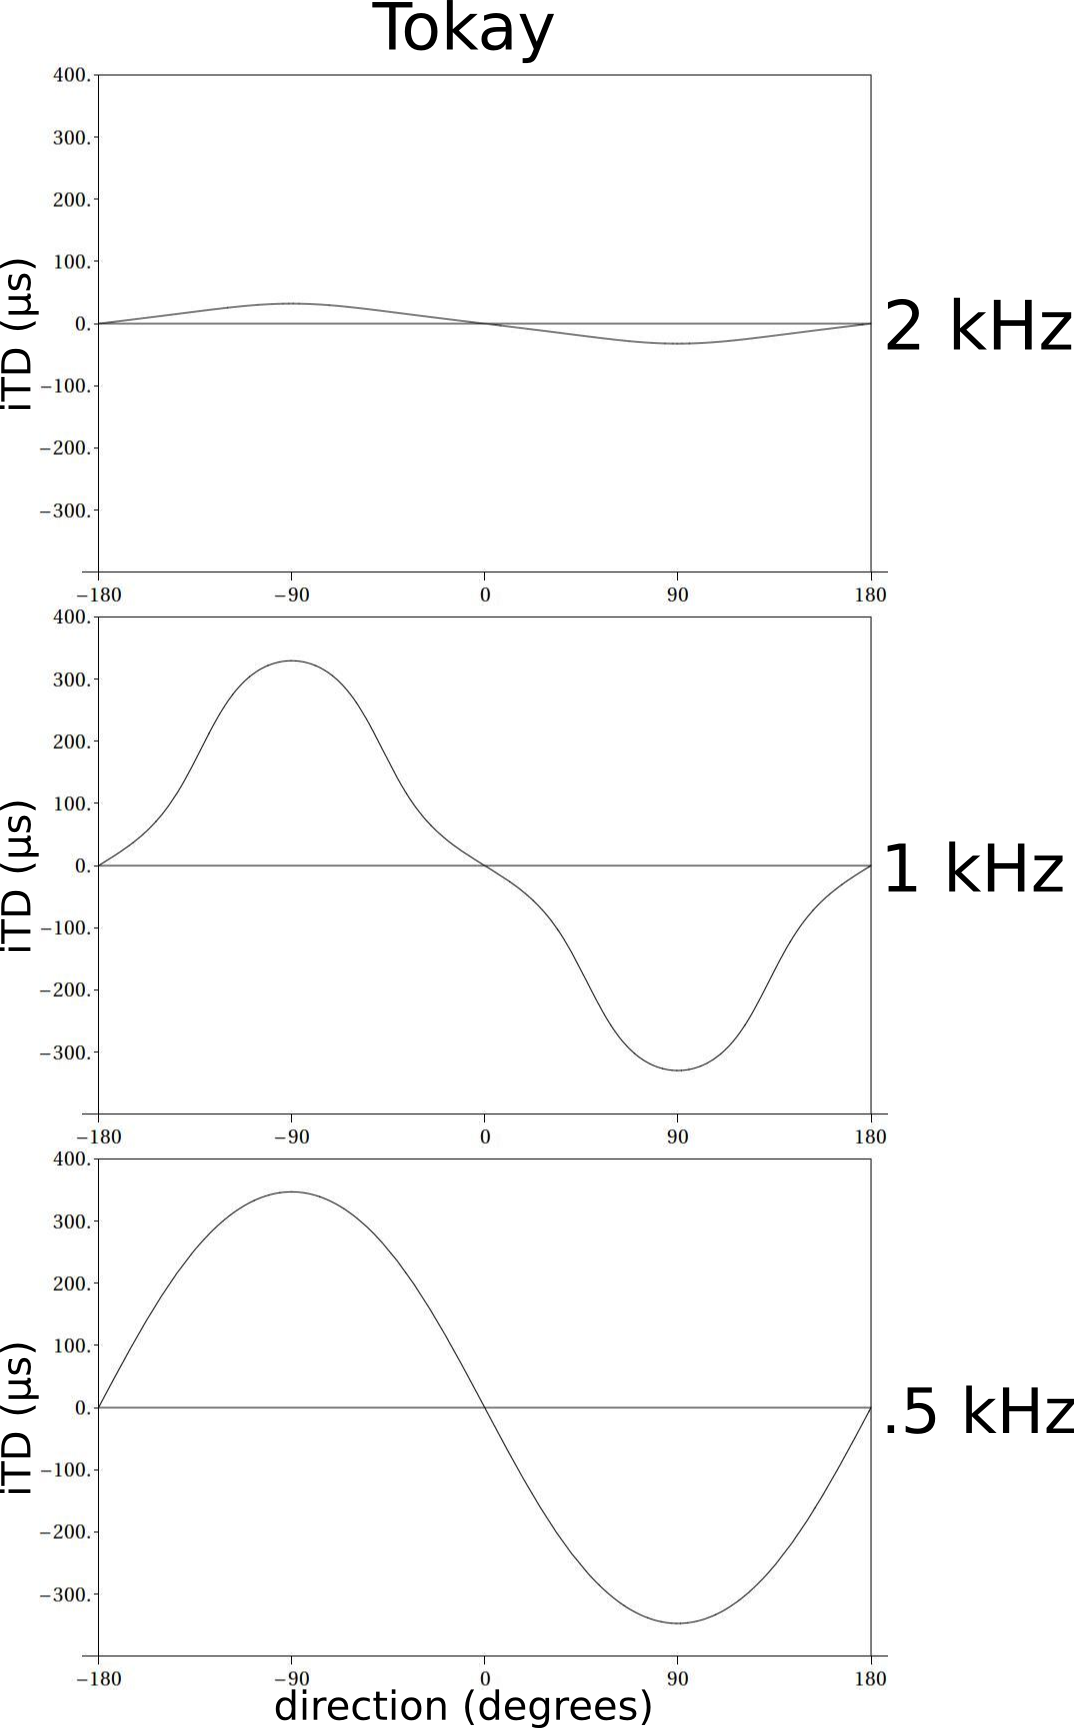
\includegraphics[width = 3.8 cm]{Diagrams/Presentation/iTDdirection.png}
\end{column}
\end{columns}
\end{frame}


\begin{frame}
\frametitle{iTD/iLD Frequency Regimes}
\begin{columns}
\begin{column}{0.5\textwidth}
\begin{exampleblock}{}
\small
 \begin{itemize}
  \item The frequency for transition from iTD to iLD based localization is determined by $f_0$.
  \item Possibility of a frequency regime where both cues can simultaneously be used.
 \end{itemize}
\end{exampleblock}
\end{column}
     \begin{column}{0.5\textwidth}
      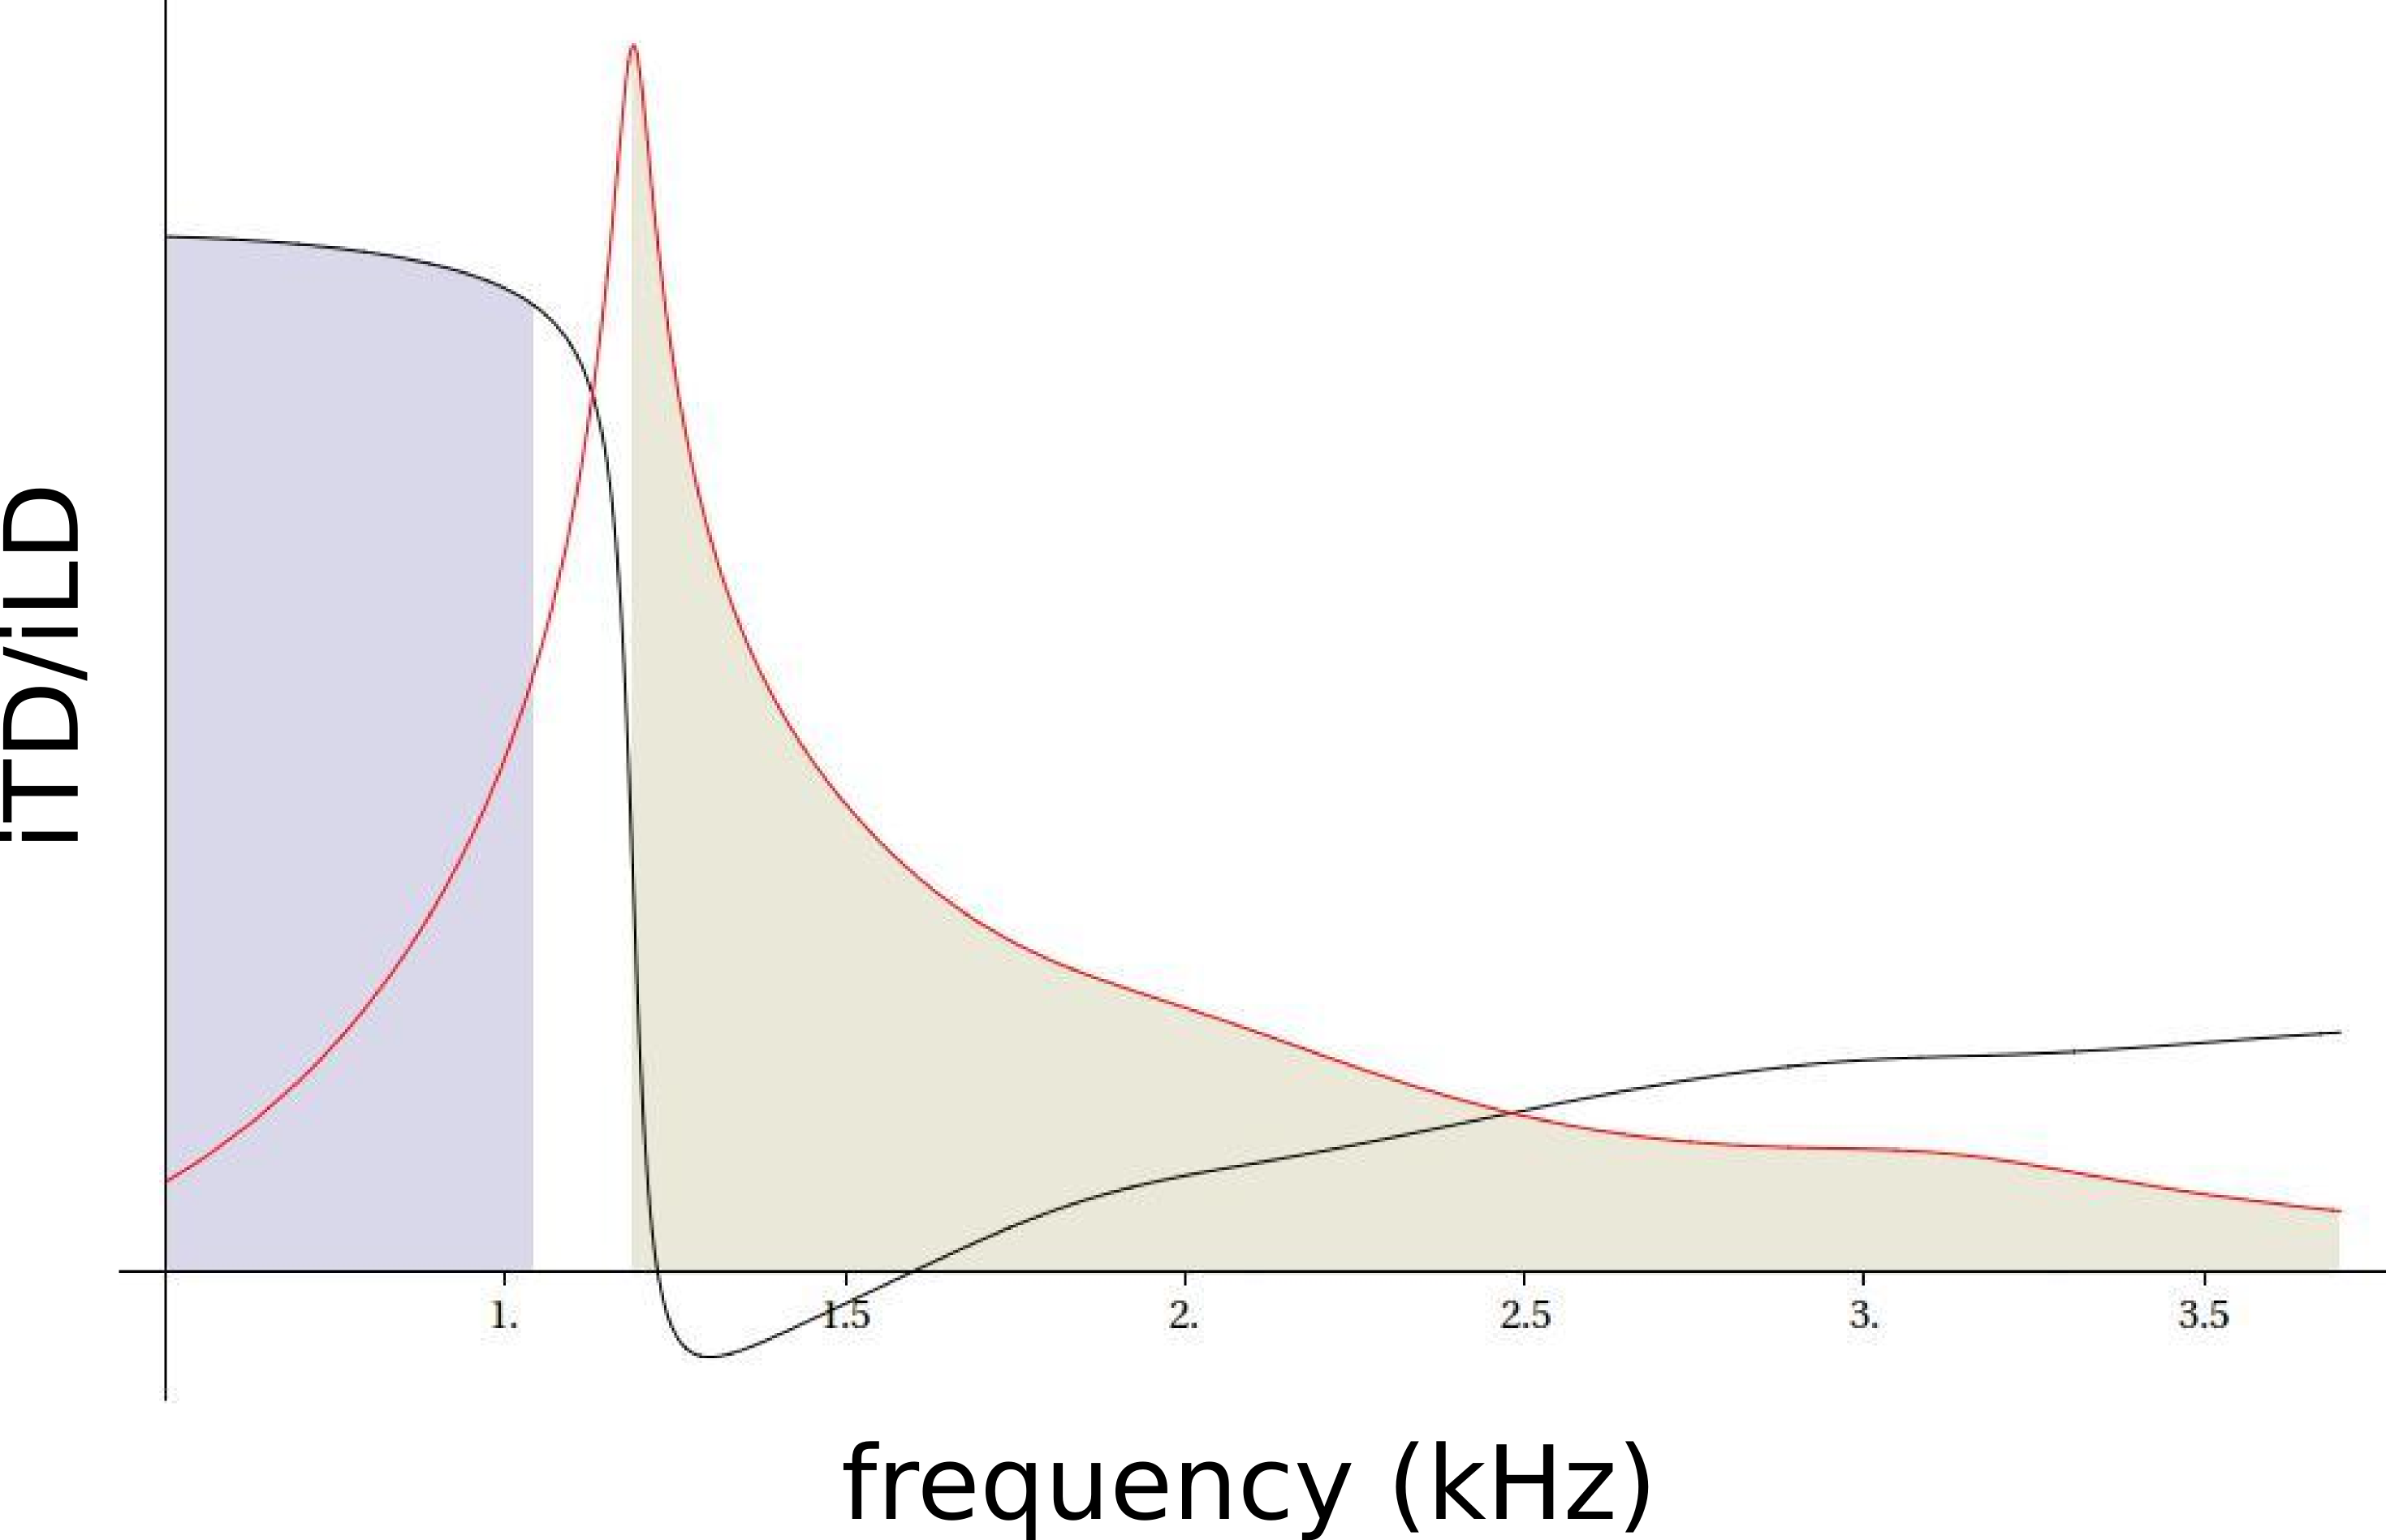
\includegraphics[width = 6 cm]{Diagrams/Presentation/tokayregions.png}
\end{column}
\end{columns}
\end{frame}

\section{Conclusion}
\begin{frame}[t]
 \frametitle{Conclusion}
\end{frame}

\begin{frame}[t]
 \frametitle{Thank You}
 \begin{figure}
  \centering
  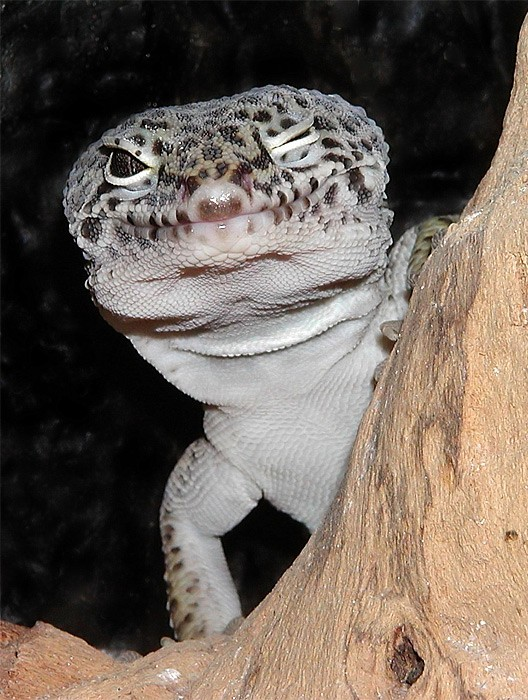
\includegraphics[width=.3\textwidth]{Diagrams/geckowink.jpg}
 \end{figure}
\end{frame}


\end{document}
